\documentclass[journal]{}                % final (journal style)
% \documentclass[review,journal]{vgtc}         % review (journal style)
%\documentclass[widereview]{vgtc}             % wide-spaced review
%\documentclass[preprint,journal]{vgtc}       % preprint (journal style)

%% Uncomment one of the lines above depending on where your paper is
%% in the conference process. ``review'' and ``widereview'' are for review
%% submission, ``preprint'' is for pre-publication, and the final version
%% doesn't use a specific qualifier.

%% Please use one of the ``review'' options in combination with the
%% assigned online id (see below) ONLY if your paper uses a double blind
%% review process. Some conferences, like IEEE Vis and InfoVis, have NOT
%% in the past.

%% Please use the ``preprint''  option when producing a preprint version
%% for sharing your article on an open access repository

%% Please note that the use of figures other than the optional teaser is not permitted on the first page
%% of the journal version.  Figures should begin on the second page and be
%% in CMYK or Grey scale format, otherwise, colour shifting may occur
%% during the printing process.  Papers submitted with figures other than the optional teaser on the
%% first page will be refused. Also, the teaser figure should only have the
%% width of the abstract as the template enforces it.

%% These few lines make a distinction between latex and pdflatex calls and they
%% bring in essential packages for graphics and font handling.
%% Note that due to the \DeclareGraphicsExtensions{} call it is no longer necessary
%% to provide the the path and extension of a graphics file:
%% \includegraphics{diamondrule} is completely sufficient.
%%
\ifpdf%                                % if we use pdflatex
  \pdfoutput=1\relax                   % create PDFs from pdfLaTeX
  \pdfcompresslevel=9                  % PDF Compression
  \pdfoptionpdfminorversion=7          % create PDF 1.7
  \ExecuteOptions{pdftex}
  \usepackage{graphicx}                % allow us to embed graphics files
  \DeclareGraphicsExtensions{.pdf,.png,.jpg,.jpeg} % for pdflatex we expect .pdf, .png, or .jpg files
\else%                                 % else we use pure latex
  \ExecuteOptions{dvips}
  \usepackage{graphicx}                % allow us to embed graphics files
  \DeclareGraphicsExtensions{.eps}     % for pure latex we expect eps files
\fi%

%% it is recomended to use ``\autoref{sec:bla}'' instead of ``Fig.~\ref{sec:bla}''
\graphicspath{{figures/}{pictures/}{images/}{./}} % where to search for the images

\usepackage{microtype}                 % use micro-typography (slightly more compact, better to read)
\PassOptionsToPackage{warn}{textcomp}  % to address font issues with \textrightarrow
\usepackage{textcomp}                  % use better special symbols
\usepackage{mathptmx}                  % use matching math font
\usepackage{times}                     % we use Times as the main font
\renewcommand*\ttdefault{txtt}         % a nicer typewriter font
\usepackage{cite}                      % needed to automatically sort the references
\usepackage{tabu}                      % only used for the table example
\usepackage{booktabs}                  % only used for the table example
\usepackage{amsmath}
\usepackage{here}
\usepackage{xcolor}
% \usepackage{url}
\usepackage{hyperref}
% \usepackage{enumerate}
\usepackage{enumitem}
%% We encourage the use of mathptmx for consistent usage of times font
%% throughout the proceedings. However, if you encounter conflicts
%% with other math-related packages, you may want to disable it.

%% In preprint mode you may define your own headline. If not, the default IEEE copyright message will appear in preprint mode.
%\preprinttext{To appear in IEEE Transactions on Visualization and Computer Graphics.}

%% In preprint mode, this adds a link to the version of the paper on IEEEXplore
%% Uncomment this line when you produce a preprint version of the article 
%% after the article receives a DOI for the paper from IEEE
%\ieeedoi{xx.xxxx/TVCG.201x.xxxxxxx}

%% If you are submitting a paper to a conference for review with a double
%% blind reviewing process, please replace the value ``0'' below with your
%% OnlineID. Otherwise, you may safely leave it at ``0''.
\onlineid{1023}

%% declare the category of your paper, only shown in review mode
\vgtccategory{Research}
%% please declare the paper type of your paper to help reviewers, only shown in review mode
%% choices:
%% * algorithm/technique
%% * application/design study
%% * evaluation
%% * system
%% * theory/model
\vgtcpapertype{application/design study}

%% Paper title.
\title{TimeTubesX: Query-Driven Visual Exploration of\\Observable and Recurring Time Variation Patterns of Blazars}

%% This is how authors are specified in the journal style

%% indicate IEEE Member or Student Member in form indicated below
% \author{Roy G. Biv, Ed Grimley, \textit{Member, IEEE}, and Martha Stewart}
\author{Naoko Sawada,~%\IEEEmembership{Student member,~IEEE,}
        Makoto Uemura,~%\IEEEmembership{}
        Johanna Beyer,~%\IEEEmembership{Member,~IEEE}
        Hanspeter Pfister,~%\IEEEmembership{}
        and~Issei~Fujishiro}
\authorfooter{
%% insert punctuation at end of each item
\item
 N. Sawada is with Keio University and Harvard University. 
 \newline E-mail: naoko.sawada@fj.ics.keio.ac.jp.
\item
 M. Uemura is with Hiroshima University. 
 \newline E-mail: uemuram@hiroshima-u.ac.jp.
\item
 J. Beyer and H. Pfister are with Harvard University. 
 \newline E-mail: {jbeyer, pfister}@g.harvard.edu
\item 
 I. Fujishiro is with Keio University and Hangzhou Dianzi University. 
 \newline E-mail: fuji@ics.keio.ac.jp.
}

%other entries to be set up for journal
\shortauthortitle{Sawada \MakeLowercase{\textit{et al.}}: TimeTubesX: Query-Driven Visual Exploration of Observable and Recurring Patterns of Blazars}
%\shortauthortitle{Firstauthor \MakeLowercase{\textit{et al.}}: Paper Title}

%% Abstract section.
\IEEEtitleabstractindextext{%
\begin{abstract}
Blazars are celestial bodies of high interest to astronomers. 
In particular, through the analysis of photometric and polarimetric observations of blazars, 
astronomers aim to understand the physics of the blazar’s relativistic jet. 
However, it is challenging to recognize correlations and time variations of the observed polarization, intensity, and color of the emitted light. In our prior study, we proposed TimeTubes to visualize a blazar dataset as a 3D volumetric tube. In this paper, we build primarily on the TimeTubes representation of blazar datasets to present a new visual analytics environment named TimeTubesX, 
into which we have integrated sophisticated feature and pattern detection techniques for effective location of observable and recurring time variation patterns in long-term, multi-dimensional datasets. 
Automatic feature extraction detects time intervals corresponding to well-known blazar behaviors. 
Dynamic visual querying allows users to search long-term observations for time intervals similar to a time interval of interest (query-by-example) or a sketch of temporal patterns (query-by-sketch). 
Users are also allowed to build up another visual query guided by the time interval of interest found in the previous process and refine the results. We demonstrate how TimeTubesX has been used successfully by domain experts for the detailed analysis of blazar datasets and report on the results.

% Blazars are celestial bodies of high interest to astronomers. In particular, astronomers aim to understand, through analysis of photometric and polarimetric observations of blazars, the physics of the blazar's relativistic jet. However, it is challenging to recognize time variation of and correlations among the observed polarization, intensity, and color of the emitted light. 
% We proposed TimeTubes, through which a blazar dataset is visualized as a 3D volumetric tube. In this paper, we develop TimeTubesX, a new visual analytics environment for blazar datasets that extends our previous TimeTubes. 
% In this paper, we describe TimeTubesX, a new visual analytics environment for blazar datasets that extends our previous TimeTubes, through which a blazar dataset is visualized as a 3D volumetric tube.
% We have integrated sophisticated feature and pattern detection techniques into TimeTubesX that allow for effective location of observable and recurring time variation patterns in long-term, multi-dimensional datasets. 
% Blazars are celestial bodies of high interest to astronomers. In particular, astronomers aim to understand, through analysis of photometric and polarimetric observations,
% the physics of the relativistic jet that is ejected from a blazar's center.
% However, it is challenging to recognize time variation patterns of and correlations among the observed polarization, intensity, and color of the emitted light. 
% We have previously proposed TimeTubes, through which a blazar dataset is visualized as a 3D volumetric tube.
% In this paper, we develop TimeTubesX, a new visual analytics environment for blazar observations that extends our previous TimeTubes.
% We have integrated sophisticated feature and pattern detection techniques into TimeTubesX that allow for the effective location of observable and recurring time variation patterns in long-term, multi-dimensional datasets.
% Automatic feature extraction methods detect time intervals that include well-known blazar behaviors. 
% Dynamic visual querying methods allow users to search long-term observations for time intervals similar to a time interval of interest (query-by-example) or a sketch of time variation patterns (query-by-sketch). 
% The result of a query can be directly re-used as an input for another dynamic visual query.
% This iterative pattern search allows users to build up another query guided by the interesting time interval found in the previous process and to refine results. 
% We demonstrate how TimeTubesX has been successfully used by domain experts for the detailed analysis of blazar observations and report on the results.
\end{abstract}

% Note that keywords are not normally used for peerreview papers.
\begin{IEEEkeywords}
Visual analytics, feature extraction, visual query, multi-dimensional, time-dependent visualization, astrophysics, blazar
\end{IEEEkeywords}}

%% Keywords that describe your work. Will show as 'Index Terms' in journal
%% please capitalize first letter and insert punctuation after last keyword
% \keywords{Radiosity, global illumination, constant time}

%% ACM Computing Classification System (CCS). 
%% See <http://www.acm.org/class/1998/> for details.
%% The ``\CCScat'' command takes four arguments.

\CCScatlist{ % not used in journal version
 \CCScat{K.6.1}{Management of Computing and Information Systems}%
{Project and People Management}{Life Cycle};
 \CCScat{K.7.m}{The Computing Profession}{Miscellaneous}{Ethics}
}

%% A teaser figure can be included as follows
\teaser{
  \centering
  \includegraphics[width=.99\linewidth]{vgtc_journal_latex/figures/workflowGray.pdf}
  \caption{Visual exploration framework of TimeTubesX. Users can load multiple datasets into a single exploration session through visual data fusion. (A)~Users specify a query to extract features of interest; (B)~Query results are sorted by relevance; (C)~Individual results can be analyzed in high detail and compared to each other; (D)~An extraction result can be re-used as an input for a new visual query; and (E)~Users can visually explore the results in the TimeTubes and scatterplots views.}
  \label{fig:framework}
}

%% Uncomment below to disable the manuscript note
%\renewcommand{\manuscriptnotetxt}{}

%% Copyright space is enabled by default as required by guidelines.
%% It is disabled by the 'review' option or via the following command:
% \nocopyrightspace


\vgtcinsertpkg

%%%%%%%%%%%%%%%%%%%%%%%%%%%%%%%%%%%%%%%%%%%%%%%%%%%%%%%%%%%%%%%%
%%%%%%%%%%%%%%%%%%%%%% START OF THE PAPER %%%%%%%%%%%%%%%%%%%%%%
%%%%%%%%%%%%%%%%%%%%%%%%%%%%%%%%%%%%%%%%%%%%%%%%%%%%%%%%%%%%%%%%%

\begin{document}

%% The ``\maketitle'' command must be the first command after the
%% ``\begin{document}'' command. It prepares and prints the title block.

%% the only exception to this rule is the \firstsection command
\firstsection{Introduction}\label{sec:introduction}
\maketitle
\ifCLASSOPTIONcompsoc
\IEEEraisesectionheading{\section{Introduction}\label{sec:introduction}}
\else
\section{Introduction}
\label{sec:introduction}
\fi
% Blazar are an important topic of researches in astronomy and high-energy astrophysics. 
\IEEEPARstart{B}{lazars} are important to the studies of astronomy and high-energy astrophysics. 
They are in a class of extremely bright galactic nuclei called active galactic nuclei (AGN) that shoot out a stream of particles from their center~\cite{Antonucci1993a}. 
A relativistic jet is angled directly toward the Earth from a central black hole of a blazar (see Fig.~\ref{fig:blazar}).
However, relatively little is known about the intricate physics of these jets' structures. %about these structures.
% To demystify the intricate physics of the jet's structures,
Astronomers pay careful attention to blazars
because the jet radiation of blazars is more amplified than that of other AGN.
% Astronomers pay careful attentions to blazars
%Blazars are a class of extremely bright galactic nuclei with a supermassive black hole at their center~\cite{Antonucci1993a}. 
%They emit a relativistic jet directly angled toward the Earth, 
%as illustrated in \autoref{fig:blazar}.
%The astronomers pay careful attentions to blazars 
%because the physics of the jet is mysterious even nowadays.
% To predict the effects of the magnetic field on the jet,
To demystify the jets' structures,
astronomers need to analyze correlations and time variations in photometric and polarimetric observations of the emitted light.
% of observed polarization, intensity, and color of the emitted light.
% However, it is challenging for them to manually identify recurring patterns or similar time intervals from long-term, multi-dimensional observations.
%for effectively understanding dynamic variations in and feature causality among multiple variables.
%Our previous application provides visual data fusion for datasets from multiple observatories and diverse interactions
%to accomplish more effective data analysis~\cite{Fujishiro2018}.
%To identify known blazar behaviors or recurring patterns, astronomers need to meticulously analyze their high-dimensional data.
For instance, a light burst (i.e., \textit{flare}) is one of the most distinctive behaviors of blazars~\cite{Bednarek1999, Atoyan2001}.
Identifying flares requires astronomers to scrutinize correlations of the emitted light's intensity with polarization and/or color, because looking at the time variation of the intensity alone is insufficient. %always varies finely.
%
In addition to flares, some astronomers are interested in the polarization direction of light and whether it rotates~\cite{Marscher2008, Uemura2017}.
%In addition to flares, some astronomers reported that the polarization direction of the light sometimes rotates~\cite{Marscher2008, Uemura2017}.
It is a controversial question in astronomy whether such \textit{rotations} are real or due to random variations of polarization.
To verify polarization rotations, correlations of the polarization with the intensity and/or the color are crucial.
% Moreover, astronomers would like to locate time intervals with common features in time variations.
Moreover, astronomers would like to locate time intervals with common features in  time variations
to understand what happens inside the jet.
However, it is an overwhelming process for them to manually examine all time intervals in long-term, multi-dimensional datasets in order to detect these significant patterns and validate hypotheses.
%those including flares/rotations and validating a specific hypothesis.

To support these exploration challenges, 
we have developed \textit{TimeTubesX}, a new visual analytics environment for blazar observations. 
%
This novel system extends our previous visualization scheme, called \textit{TimeTubes}~\cite{Fujishiro2018}, 
which allows users to interactively explore multi-dimensional, time-dependent observation datasets of blazars in a unique 3D tube view and to combine datasets from multiple observatories into a single visualization session termed \emph{visual data fusion}.
%, which focused on visualizing blazar observations in a unique 3D view.
%
%that integrates our previous TimeTubes view.
%Previously, we proposed \textit{TimeTubes}~\cite{Fujishiro2018}, a unique 3D visualization for blazar observations that allowed users to interactively explore their high-dimensional datasets more intuitively, and to combine datasets from multiple observatories into a single visualization session.
%on top of the previous TimeTubes.
In TimeTubesX, we place more focus on visual analysis and automated and semi-automated approaches for feature and pattern detection.
%We have developed advanced feature extraction mechanisms for TimeTubesX, consisting of automatic and interactive approaches.
The automatic feature extraction methods, which are in part an extension of our previous work~\cite{Sawada2018}, detect time intervals corresponding to well-known blazar behaviors, such as flares and rotations.
%with reference to the astronomers' reports,
The dynamic visual querying methods, on the other hand, are useful for analysis and detection of recurring patterns that have not yet been explored in detail. 

% This paper extends our previous short paper about the automatic feature extraction for blazar observations~\cite{Sawada2018}, but we have significantly improved our detection algorithms. 
% The primary contributions of this paper are three-fold. 
Our first contribution is a detailed goal and task analysis performed with domain experts to design a visual analytics framework for blazar observations. 
Subsequently, we have designed and implemented TimeTubesX as a web-based and open-source system. 
Our second contribution lies in powerful automatic feature extraction methods for well-known blazar behaviors and an intuitive visual query platform for multi-dimensional, time-dependent data.
Finally, as our third contribution, we demonstrate the usefulness of TimeTubesX through experiments with a synthetic dataset, real data analyses, and feedback from domain experts.
We envision that our visual query mechanisms could be applied to multi-dimensional, time-series datasets in other domains to help users identify recurring patterns or similar time intervals.
% \begin{itemize}
%     \item %Implementation of a new web-based visual analysis environment,termed TimeTubesX, for blazar observations based on analysis ofspecific sets of domain goals and involved tasks.
%     A detailed goal and task analysis performed with our domain experts to design a visual analysis framework for blazar observations. 
%     Subsequently, we have designed and implemented TimeTubesX as a web-based and open-source system. 
%     \item Powerful automatic feature extraction methods for well-known blazar behaviors and an intuitive visual query platform for time-dependent, multi-dimensional data.
%     \item A demonstration of the usefulness of TimeTubesX based on a real data analysis by a domain expert.
% \end{itemize}
%We fully improved the detection algorithms.

% We first review related work
% in \autoref{sec:relatedWork}, before describing our target data and domain goals and tasks in \autoref{sec:domainAnalysis}.
% \autoref{sec:systemDesign} introduces the system design of TimeTubesX.
% \autoref{sec:automaticExtraction}, \autoref{sec:visualQuery}, and \autoref{sec:otherFunctions} present details on our feature and pattern detection methods.
% We demonstrate the effectiveness of the proposed intuitive feature extraction through an evaluation case in \autoref{sec:evaluation}.
% In \autoref{sec:discussion}, we discuss feedback from domain experts and limitations of TimeTubesX.
% We conclude this paper in \autoref{sec:conclusion}.



% For example, the black hole ejects a jet almost at the speed of light, 
% but what accelerates it is not clear yet.

% if they look over animated scatterplots, 
% which have been commonly used in the astrophysical community.

% Regarding the behaviors of blazars, there are a lot of mysterious parts. 
% When the relativistic jet in a blazar forms a burst, the light from a blazar gets highly luminous, that is called a flare. 
% Flare is one of the most characteristic behaviors. 
% Some astronomers report that the polarization direction of the light from blazars sometimes rotates. 
% However, it is controversial in astronomy whether the rotations are real ones or fake ones caused by random variations of polarization.
% To verify polarization rotations, astronomers need to scrutinize correlations among other observation variables. 
% On the other hand, there can exist undiscovered phenomena of blazars. 
% It is significant to explore recurring patterns of time variations or correlations among variables. 
% Nevertheless, deliberate analysis across multiple variables is indispensable.
% To address these difficulties, we introduce a novel feature extraction for blazar observations.
% It supports two types of feature extraction: Automatic extraction and visual query. 
% The automatic extraction can squeeze only observable time intervals from (multiple) long-term observations, 
% whereas the visual query can find time intervals similar to a region of interest (ROI) or shape of interest (POI). 

% When the relativistic jet in a blazar forms a burst, the light from a blazar gets highly luminous, that is called a flare. 

% In other words, there are too many peaks of the intensity to identify notable flares 
% without regard for correlations between the intensity and other parameters.

% It takes time to visit all time intervals to find flares or rotations and inspect correlations among the other parameters.

% this paper presents a feature extraction for blazar observations as an advanced function of TimeTubes, 
% which offers the astronomers time intervals including known blazar phenomena, such as flares and rotations, 
% and those similar to a region or shape of interest.
% The feature extraction provides two approaches: automatic and interactive.

%about visualization techniques for astronomical data and feature extraction techniques 
\section{Related work\label{sec:relatedWork}}
Our target blazar datasets are multi-dimensional (mD), semi-structured, and time-dependent.
This section reviews prior work in astronomical visualization and visual query systems for mD and time-series data. 


\subsection{Visualization for Astronomical Data}\label{sec:relatedAstronomy}
Most astronomers work on analyzing signals from distant celestial bodies measured from the Earth~\cite{Kent2017}. 
%Astronomers make much account of observing and analyzing signals from distant celestial bodies
%because they cannot travel just to see the bodies with their naked eyes~\cite{Kent2017}.
% Li et al.~\cite{Li2007} visualize positional and data-inherent uncertainties of large-scale 3D astronomical simulations.
% For multi-wavelength astronomical data, Li and Hanson~\cite{Li2008} propose a system for visual analysis across multiple datasets.
% %Li and Hanson~\cite{Li2008} tackle 3D visualization for multi-wavelength astronomical data from multiple data sources, which realizes easy visual analysis across multiple datasets.
% Baines et al.~\cite{Baines2017} develop a web-based data discovery portal, ESASky, for exploring multi-wavelength sky data.
% GalStamps~\cite{McCurdy2019} is a visual analytics tool for both real and simulated galaxy observations,
% which realizes analysis across multiple different visualization, such as scatterplots and parallel coordinate plots.
% Though many techniques have been developed for astronomical data, there are no other effective techniques for blazar observations, except for our early attempt~\cite{Fujishiro2018}.
ESASky~\cite{Baines2017} and OpenSpace~\cite{Bock2020} provide views for parts of the sky that are integrated from multiple data sources.
Almryde et al.~\cite{Almryde2016} visualize the temporal evolution of the position, mass, and radial velocity of dark matter halos. 
% Various types of telescopes are used to observe the sky or particular celestial bodies in different wavelengths 
% because visible light observation does not provide enough data to appreciate the nature of the universe.
% observing only visible light is not enough to appreciate the real nature of the universe.
Li et al.~\cite{Li2008} realize simple visual analysis across multi-wavelength datasets.
IGM-Vis~\cite{Burchett2019} is a visual analytics tool for quasar sightline data.
% propose 3D view for galaxies and quasar sightlines and 2D views for spectrum for the analysis of intergalactic medium and circumgalactic medium.
Some approaches~\cite{Haroz2008, Li2008, Preston2016, McCurdy2019, Burchett2019} provide linked-view visualization systems that allow users to explore multiple types of visualizations for deeper analyses.
Many techniques have been developed for the analysis of astronomical data, 
but typically, blazar researchers have used animated scatterplots (see Section~\ref{sec:VisualEncoding}) 
because there were no other effective techniques for blazar observations prior to our early attempt, TimeTubes~\cite{Fujishiro2018}.
% For more efficient data analysis with TimeTubesX, we introduce feature and pattern detection methods for blazar datasets, a part of which is an extension of our previous paper~\cite{Sawada2018}.

\subsection{Visual Queries}\label{sec:relatedFeature}
Visual query systems allow users to intuitively search for patterns of interest in their data.
%The two most common options are \emph{query-by-example} and \emph{query-by-sketch}.
%Query-by-example and query-by-sketch interfaces are powerful approaches to querying data intuitively. 
Query-by-example aims to find data samples that are similar to a user-specified example,
% However, they do not address how to find the initial interesting data samples. 
whereas query-by-sketch allows users to directly draw the shape of interest.
% , yet the techniques have to deal with the user-introduced uncertainties of sketches.

\textsf{Query-by-example.\ }
% QBE for univariate data
%In these systems, users select an example from their data, that serves as the query for the rest of the dataset.% excerpt a part of time series for their query.
Hochheiser and Shneiderman~\cite{Hochheiser2004} propose TimeSearcher, a visual exploration tool for time-series data. Users can select portions of timelines by using rectangular widgets~\cite{Buono2005, Buono2008}.
% such as Timeboxes~\cite{Buono2005} and Search Boxes~\cite{Buono2008}.
%where the users are allowed to select portions of timelines by putting boxes, termed Timeboxes~\cite{Buono2005} or Search Boxes~\cite{Buono2008}.
Holz and Feiner~\cite{Holz2009} propose a relaxed selection technique for time intervals through which users define the level of similarity either by the input speed or by spatial deviation from an original timeline.
The idea of detecting the input speed was adopted for our sketching interface.
However, these interactions are geared only toward univariate time-series data and are not appropriate for our mD blazar data.
%
%to allow ones to select a time interval and to define the level of similarity simultaneously
%by detecting either sketching speed or spatial deviation from an original timeline.
%Their interactions work effectively only for univariate time-series data.

% QBE for multivariate data
Query-by-example methods for mD data have also been proposed.
Martin and Ward~\cite{Martin2005} describe brushing techniques for visualizations,
such as scatterplots matrices and parallel coordinate plots.
Elmqvist et al. propose interactions for constructing visual queries with star plots~\cite{Elmqvist2007} and multiple scatterplots~\cite{Elmqvist2008}.
Scribble query~\cite{Nielsen2016} allows users to form visual queries by scribbling axes of parallel coordinate plots.
% introduces a touch interaction method for forming visual queries
% through parallel coordinate plots by scribbling axes. 
Several works have focused on unstructured mD datasets~\cite{Martin2005,Elmqvist2007,Nielsen2016}, 
%The techniques in \cite{Martin2005}, \cite{Elmqvist2007}, and \cite{Nielsen2016} effectively work for unstructured mD datasets, 
but they are not versatile enough to examine correlations among our idiosyncratic variables (see Section~\ref{sec:BlazarData}), and they do not support queries for structured time-series data.
The scatterplots by Martin and Ward~\cite{Martin2005} and Elmqvist et al.~\cite{Elmqvist2008} can be partially useful for structured data, but they cannot be applied to time-series data.

% QBS
\textsf{Query-by-sketch.\ } 
%Users may sketch the shape of interest for their query.
Early examples of query-by-sketch tools include QuerySketch~\cite{Wattenberg2001} for temporal databases and QueryLines~\cite{Ryall2005} for multiple timelines. 
%QuerySketch~\cite{Wattenberg2001} is a sketch-based visual query tool for a temporal database.
%QueryLines~\cite{Ryall2005} allows the users to draw a query involving soft constraints and preferences.
TimeSketch~\cite{Eichmann2015} supports pen- and touch-based query specification but focuses only on univariate time-series data.
% symbolic approximation
%Query-by-sketch interfaces have to handle ambiguities of hand-drawn sketches. 
To manage the ambiguities of hand-drawn sketches, several systems discretize the query and datasets into symbolic or quantized representations~\cite{Muthumanickam2016,ruta2019sax}.
%The input query and time series are discretized into symbolic representations to cope with uncertainties of a hand-drawn sketch in \cite{Muthumanickam2016} and \cite{ruta2019sax}.
%
Alternatively, Correll and Gleicher~\cite{Correll2016} define invariants for sketches. % to deal with uncertainties of sketches. 
Qetch~\cite{Mannino2018} provides a matching algorithm that takes human sketching errors into account.
Our query-by-sketch interface uses sketching interactions similar to those of Qetch~\cite{Mannino2018}.
% The sketching interactions of Qetch~\cite{Mannino2018} inspired our query-by-sketch interface.
Both techniques target univariate time-series data.
%
Shao et al.~\cite{Shao2014} introduce sketch-based queries for large sets of scatterplots,
in which the system supports users with shadow-drawing suggestions. %, which we use as an inspiration for our fact-driven querying\autoref{sec:factDrivenQuerying}.
The suggestions allow users to draw a pattern based on actual values rather than their imaginations.
We use this idea as inspiration for our fact-guided querying (see Section~\ref{sec:factDrivenQuerying}).
%users are allowed to draw a pattern with the help of shadow-drawing suggestions,
%due to which the input sketch is not just a fiction by the users but based on fact.
%It influences the concept of our fact-driven querying, as discussed in \autoref{sec:factDrivenQuerying}.
While these systems support querying structured mD data, they cannot be applied to time-series data.

% QBS for volume data
Several sketch-based techniques for multi-scalar volume data allow users to select regions of a 3D object through an ordinary 2D painting tool.
The techniques by Owada et al.~\cite{Owada2005} and Igarashi et al.~\cite{Igarashi2016} extract a plausible 3D region from the volume
by following contours or isosurfaces, respectively.
Tzeng et al.~\cite{Tzeng2003} present an method for specifying high-dimensional classification functions for the volume
by brushing regions of interest. % and those of uninterest.
BrainGazer~\cite{Bruckner2009} provides simple interactions for the selection of a region of interest in the volume
using drag-and-drop functionality.
% clicking on and dragging a 3D object. 
These techniques can only target multi-scalar volume data. 

\textsf{Combinations of query-by-example and query-by-sketch.\ }
Query-by-example techniques do not address how to find the initial data samples of interest, 
% users have to first identify an interesting data point in their dataset,
while query-by-sketch techniques must surmount the user-introduced ambiguities of sketches.
Combining both styles helps to resolve this trade-off, as addressed by 
Bernard et al.~\cite{Bernard2010} and Lee et al.~\cite{Lee2019}. 
The system formulated by Bernard et al.~\cite{Bernard2010} supports univariate time-series data, while the one by Lee et al.~\cite{Lee2019} supports unstructured time-series data.
% To get the best of both worlds, TimeTubesX supports automatic feature extraction as wells as query-by-example and query-by-sketch interactions.
To get the best of both worlds, TimeTubesX supports both types of querying interactions.
%
%To compensate these shortcomings, 
%we go together with both styles to build a new integrated feature extraction system 
%with both styles.

% because standard visualizations like scatterplots, star plots, parallel coordinate plots is not enough 
% for the astronomers to understand correlations among idiosyncratic variables (see Sec.~\ref{sec:BlazarData}) to build their query.


% % QBE for univariate data
% There are many query-by-example techniques which can deal with univariate datasets.
% Hochheiser and Shneiderman~\cite{Hochheiser2004} propose a visual exploration tool for time-series data, named TimeSearcher,
% where users are allowed to select portions of timeline by putting boxes, Timeboxes~\cite{Buono2005}.
% Search Box~\cite{Buono2008}, an augmented version of Timebox, allows users to change the shape of the selected pattern 
% and provides a series of characteristic patterns to prune timelines. 
% % SOMFlow~\cite{Sacha2018} is a visual analytic tool which can interactively refine clusters based on query-by-example using self-organizing maps.
% Holz and Feiner~\cite{Holz2009} propose a relaxed selection technique for time-series data.
% The technique allows users to select a time interval and define the level of similarity simultaneously
% by detecting either sketching speed or spatial deviation from an original timeline.
% These methods are effective only for univariate datasets, 
% so their interactions can not be directly applied to multivariate datasets.

% % QBE for multivariate data
% There also exist query-by-example methods for multivariate non-time-varying datasets.
% Martin and Ward~\cite{Martin2005} describe the design of brushing techniques for multi-dimensional data with various visualizations, 
% like scatterplot matrices, parallel coordinate plots, and the like.
% DataMeadow~\cite{Elmqvist2007} also provides interactions for constructing visual queries for multi-dimensional data 
% with star plots by adding filtering constraints to each axis of star plots. 
% Elmqvist et al.~\cite{Elmqvist2008} propose a new interface for interactively building queries for a multi-dimensional dataset 
% by providing smooth transition animation between scatterplots in a similar way to rolling a dice. 
% Scribble query, proposed by Nielsen et al.~\cite{Nielsen2016}, introduces a touch interaction 
% for visually forming queries for a multi-dimensional dataset
% through parallel coordinate plots by scribbling axes to select categories or ranges.
% They can deal with non-time-varying multivariate datasets, 
% but standard visualizations like scatterplots, star plots, parallel coordinate plots is not enough 
% for astronomers to understand correlations among idiosyncratic variables (see Sec.~\ref{sec:BlazarData}) to build their query.



% As detailed in Sec.~\ref{sec:BlazarData},
% in the target blazar datasets of TimeTubesX, 
% two structured polarization parameters describe linear polarization of the light
% and two retinal parameters explain the brightness and color.
% In other words, 

% Astrophysics can be said to be the ultimate remote sensing,

% Visualizations for simulated data have been extensively studied in astronomy.
% Haroz et al.~\cite{Haroz2008} visualize multiple simulation results,
% where they colorize particles to express uncertainties in time-varying cosmological particle data.
% Kahler et al.~\cite{Kahler2002a} render simulations of the evolution of the first star in the universe.
% The gas distribution is expressed by opacities, whereas temparature is by colors.
% Jensen et al.~\cite{Jensen2001} present a physical model of the night sky seen on the Earth.
% Genetti~\cite{Genetti2002} simulates and visualizes Orion Nebula from various viewpoints.
% Magnor et al.~\cite{Magnor2005} present an interactive visualization tool for realistically rendered dust distributions around illuminating stars.

% We present visualizations for observed or measured data in astronomy.
% McDonald and Montgomery~\cite{McDonald2012} visualize high-resolution laser altimeter data of the Moon.
% By utilizing a colormap optimized by a combination of hue and brightness,
% users are allowed to distinguish high and low altitude place.
% Additionally, the system enables users to measure the distance and slope of the lunar surface interactively.

% EASYSky visualizes multiple archives and allows users to visually identify the data source.
% OpenSpace~\cite{Bock2020} is an integrated environment for data from both observed and simulated data,
% to interactively explore the known universe.
% and supports research in astronomy and space science as well as science communication in educational situations.

% consisting of structured properties for the polarization of the light and retinal properties for the intensity and color.

% Feature extraction results in eliciting useful information from large or long-term data~\cite{Laxman2006}.
% Many methods for finding out patterns or outstanding time variations are proposed~\cite{WarrenLiao2005, Zhang2005, Rosner1983, Palshikar2009}.
% These methods may partially be effective for blazar observation datasets,
% however, the astronomers have to carefully analyze correlations among variables 
% to inspect whether the time interval is notable or not
% even after applying such methods.
% Regarding flares, only applying peak detection methods or outlier detection methods is insufficient  
% because the intensity of a blazar always varies finely in the short term.
% % Regarding rotation events of polarization, 
% % astronomers analyze a time variation of the polarization angle.
% To find out rotations of the polarization, 
% the astronomers manually track time variation of the polarization angle ($PA$), given as Eqn.~(\ref{equ:PA}), 
% as explained in analysis examples of previous reports~\cite{Ikejiri2011, Uemura2017},
% where $PA$ variation identifies only rotations around the origin. %of the Stokes plane.
% Therefore, a new method is desired, which realizes easy access to and verification of candidates of remarkable time intervals.

% In query-by-example, users excerpt a part of time series for their query, 
% whereas in query-by-sketch, they sketch the shape of interest for their query.
% The following parts present prior research challenges in each of the styles.

% The following parts of this section review past attempts to visually specify a query 
% to present motivations for our work.

% Many query-by-example techniques can deal with univariate time-series datasets.
% Search Box~\cite{Buono2008}, an augmented version of Timebox, allows users to change the shape of the selected pattern 
% and provides a series of characteristic patterns to prune timelines.

% DataMeadow~\cite{Elmqvist2007} also provides interactions for constructing visual queries for mD data 
% with star plots by adding filtering constraints to each axis of star plots. 
% Elmqvist et al.~\cite{Elmqvist2008} propose a new interface for interactively building queries for mD data 
% by providing smooth transition animation between scatterplots in a way similar to rolling a dice.

% but obviously, they cannot be applied to time-series data, either.

% Many sketch-based querying systems are developed for univariate time-series data.

% where users are allowed to draw the shape of a pattern for a query.
% It simply computes Euclidean distance between a sketch and time series in a database.
% It prunes plots according to the soft constraints and orders the selected plots by the extent to which they satisfy preferences. 
% It computes similarities between a query and time series in three different distance metrics:
% Euclidean distance, dynamic time warping~\cite{Berndt1994}, and spatial assembling distance~\cite{Chen2007},
% and creates a human-annotated ranking based on crowd-sourcing evaluations.
% According to their experimental results, the dynamic time warping produces the closest ranking to the human-annotated ranking. 
% Therefore, we choose the dynamic time warping in the similarity measurement process in the proposed visual query.

% A single sketch can be produced under different mental models.
% Comparing a user-drawn sketch and time series in a symbolic space can conduct a fuzzy pattern search.
% Muthumanickam et al.~\cite{Muthumanickam2016} define shape grammars composed of thirteen basic elementary shapes 
% to approximate data with the predefined symbols.
% Symbolic Aggregate approXimation (SAX)~\cite{Lin2007} is a symbolic representation for time series.
% SAX Navigator, proposed by Ruta et al.~\cite{ruta2019sax}, is a visual exploration tool for a large collection of univariate time series based on SAX representations.
% Users query a pattern of interest as a SAX letter sequence by clicking a cell on a grid. 
% Other approaches to deal with uncertainties of sketch
% The prototype query system, named QuerySketch, can take account of the invariants in the matching process.
% present Qetch,
% which is a tool to query time series based on a user-drawn sketch as well.
% It provides a matching algorithm taking human sketching errors into account.
% The background algorithms of QuerySketch and Qetch take uncertainties of the sketch into account.
% To deal with uncertainties of sketches, Shao gives suggestions for drawing 

% Owada et al.~\cite{Owada2005} propose a simple and intuitive interface 
% for volume segmentation, named Volume Catcher.
% Users trace a contour of the volume and then the system automatically extracts a plausible 3D region inside the input stroke.
% Igarashi et al.~\cite{Igarashi2016} propose an environment 
% where users are allowed to select a region of the volume by interactions like an ordinary 2D painting tool.
% The main difference between the two systems is 
% The sketching interactions in~\cite{Owada2005} work on a contour of the volume
% while those in~\cite{Igarashi2016} work on isosurfaces in the volume.
% which they do not with simple sketching interactions.
% They need to paint only on a couple of slices of the volume to classify the entire volume.% unlike the semi-structured and time-dependent mD data in TimeTubesX.
% but they inspire the interactions for selecting a part of a 3D tube in query-by-example, as detailed in Sec.~\ref{sec:QBE}.

% The visual query system in~\cite{Bernard2010} enables users to decide whether to sketch a query by hand or 
% to pick up an example pattern from a dataset, predefined shapes, or a visual catalog of time series provided by the self-organizing map algorithm.
% On the other hand, 
% the system in~\cite{Lee2019} allows users to utilize a resulting visualization as an input pattern and to draw a sketch with reference to an actual data pattern like the shadow-drawing suggestions in~\cite{Shao2014}.
% However, these are also only for univariate datasets.
\section{Domain Analysis}\label{sec:domainAnalysis}
In this section, we specify our blazar observation data and define domain-specific goals and visualization tasks that were identified in consultation with our domain experts. 

\subsection{Blazar Observation Data}\label{sec:BlazarData}
Multiple observatories worldwide collect blazar data; however, their observed properties or units of measurement differ depending on the telescopes being used. 
To reduce uncertainties due to missing observational data and observation errors,
TimeTubesX allows users to fuse multiple datasets for the same blazar from different observatories 
through the automatic handling of potentially different definitions of observed variables~\cite{Fujishiro2018}.
Thus, users can, for example, include data from Hiroshima University and the University of Arizona in the same visualization session. 
TimeTubesX is designed to primarily process datasets acquired by Hiroshima Astrophysical Science Center at Hiroshima University,
which uses a $1.5\mathrm{m}$ Kanata telescope. 

% Observation datasets
The photometric and polarimetric datasets of Hiroshima University include six time-dependent variables: $q$, $u$, $\epsilon_q$, and $\epsilon_u$ for the observed polarization of the light (Fig.~\ref{fig:blazar} (A)), $I$ for the observed intensity (Fig.~\ref{fig:blazar} (B)), and $C$ for the observed color (Fig.~\ref{fig:blazar} (C)).
Linear polarization is represented by $Q$ and $U$, the so-called \textit{Stokes} parameters.
We mainly use fractional values of $Q$ and $U$ where $q = Q / I$ and $u = U / I$, 
because $q$ and $u$ describe the behaviors of a blazar more effectively than $Q$ and $U$~\cite{Uemura2016}.
We call the plane composed of $q$ and $u$ the \textit{Stokes plane}.
$\epsilon_q$ and $\epsilon_u$ act as the observation errors of $q$ and $u$, respectively.
The polarization degree ($PD$) and polarization angle ($PA$) derived from $q$ and $u$ are used to describe the optical polarization.
$PD$ denotes a distance from the origin of the Stokes plane, 
while $PA$ denotes one half of the polar angle in the Stoke plane, as illustrated in Fig.~\ref{fig:blazar}~(A).

The observation frequency differs depending on observatories.
The median observation interval of Hiroshima University is once every two days.
Note that the datasets have missing data due to the rotation and/or revolution of the Earth, bad atmospheric conditions, and so on.
In this paper, we process datasets from Hiroshima University for two blazars: \emph{BL Lac} and \emph{3C 454.3}. 
The two datasets for \emph{BL Lac} contain 285 data samples in each dataset from May 2008 to December 2011, while the one for \emph{3C 454.3} contains 355 data samples from July 2008 to July 2014.

\begin{figure}[tb]
    \centering
        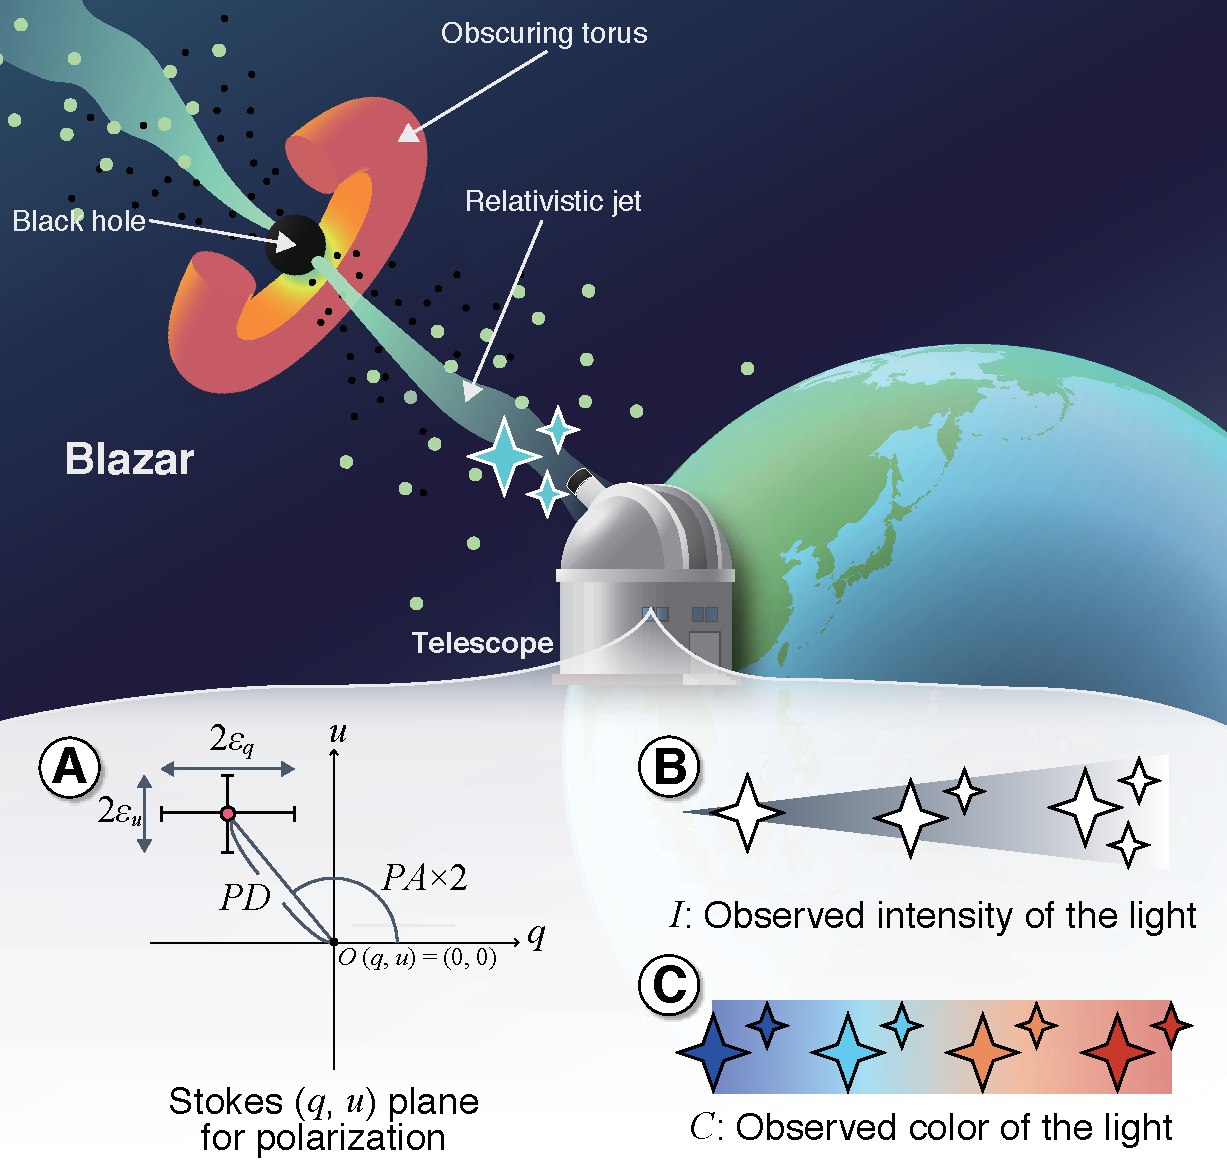
\includegraphics[width=.99\linewidth]{vgtc_journal_latex/figures/blazar_final.pdf}
    \caption{An observed blazar and its features. A blazar's central black hole emits a relativistic jet toward the Earth.
        The telescope observes its light in terms of (A) polarization, (B) intensity, and (C) color.}
    \label{fig:blazar}
\end{figure}

\subsection{Goals and Visualization Tasks}\label{sec:domainGoalsandTasks}
We interviewed two astronomers at Hiroshima University, one at Stanford University, and four at Boston University to clarify the domain goals and visualization tasks.
The main objective of these astronomers is 
to quickly extract and analyze features in temporal variations of the observed polarization, intensity, and color that are occurring at multiple time intervals. 
TimeTubesX effectively supports the following four domain goals:

\noindent\textbf{G1--Enhance the reliability of blazar observations}. 
Datasets always contain missing data and observation errors. 
Astronomers need to assess whether what they have found is plausible by analyzing the length of missing data periods and the size of errors.

\noindent\textbf{G2--Identify flares and rotations}. 
Astronomers typically pay attention to time intervals with dynamic time variations,
such as flares and rotations.
The analysis of time intervals with such dynamic variations helps astronomers demystify jets' structures.

\noindent\textbf{G3--Locate recurring blazar behaviors}.
Besides well-known behaviors such as flares and rotations, 
recurring patterns or common features can also exist.
Thus, upon finding an interesting pattern or feature, 
astronomers want to locate other time intervals similar to it.

\noindent\textbf{G4--Explore time intervals validating a hypothesis of blazar behaviors}.
Through their analyses or experiences, astronomers sometimes make a hypothesis (e.g., that the flares of a blazar tend to co-occur with a specific polarization variation pattern). 
Astronomers need to address time intervals that might validate the hypothesis.

To attain these four goals, we have identified five visualization tasks that TimeTubesX should support:

\noindent\textbf{T1--Uncertainty-aware visualization.} 
Users should be able to perceive the reliability of data through visualizations. 

\noindent\textbf{T2--Analysis across datasets.} 
To compensate for missing data, 
the system must allow users to aggregate datasets for the same target from different sources.
Analyses across datasets should also be supported to address features that are common to multiple targets.

\noindent\textbf{T3--Analysis of dynamic variations.} 
Time intervals with drastic changes in a short time period and those with unusually large time variations should be automatically extracted.

\noindent\textbf{T4--Similarity analysis of a specific region/shape of interest and time intervals.} 
Users should be able to identify regions/shapes of interest (\emph{ROI}s/\emph{SOI}s) and search for similar time variation patterns at other time intervals without using complex query languages or parameter settings.

\noindent\textbf{T5--Fuzzy search for time intervals similar to a specific ROI/SOI.}
The system should provide not only exact matches between a ROI/SOI and time intervals but also fuzzy or approximate matches. 

To support \textbf{G1}, our previous work, TimeTubes~\cite{Fujishiro2018}, has already supported \textbf{T1} and \textbf{T2}.
Observation errors are encoded in the appearance of the 3D volumetric tube (\textbf{T1}).
An ellipsoidal snapshot and a white cruciform axis appear at each observation timestamp to distinguish missing data (\textbf{T1}).
Analysis across datasets (\textbf{T2}) is supported by visual data fusion, which allows users not only to aggregate multiple datasets for the same blazar but also to effectively compare multiple datasets for the same or a different blazar in a single visualization session.
In this paper, we mainly focus on feature and pattern detection methods to support the remaining three tasks (\textbf{T3}, \textbf{T4}, \textbf{T5}).
Consequently, we have designed an integrated visual analytics framework for blazar observations that supports all identified goals (\textbf{G1}--\textbf{G4}) and tasks (\textbf{T1}--\textbf{T5}).

\section{System Design\label{sec:systemDesign}}
In this section, we provide an overview of visual encoding for blazar data and the visual exploration framework of TimeTubesX.
% We introduce a 3D tube expression of our previous TimeTubes~\cite{Fujishiro2018} into TimeTubesX.

\begin{figure}[tb]
    \begin{minipage}{0.34\linewidth}
        \centering
        \includegraphics[width=.99\linewidth]{vgtc_journal_latex/figures/howtoplot.pdf}
    \end{minipage}
    \begin{minipage}{0.26\linewidth}
        \centering
        \includegraphics[width=.99\linewidth]{vgtc_journal_latex/figures/colormap.pdf}
    \end{minipage}
    \begin{minipage}{0.36\linewidth}
        \centering
        \includegraphics[width=.99\linewidth]{vgtc_journal_latex/figures/howtotube.pdf}
    \end{minipage}
    \begin{minipage}{0.34\linewidth}
        \centering
        \footnotesize{\sf (a)}
        \end{minipage}
    \begin{minipage}{0.26\linewidth}
        \centering
        \footnotesize{\sf (b)}
    \end{minipage}
    \begin{minipage}{0.36\linewidth}
        \centering
        \footnotesize{\sf (c)}
    \end{minipage}
    \caption{Spatial mapping in the TimeTubes view. 
    (a)~Observation values of polarization decide the position and shape of an ellipse;
    (b)~observation values of intensity and color colorize the ellipse with reference to a colormap; and
    (c)~the neighboring ellipses are smoothly connected in chronological order to yield a tube shape.}
    \label{fig:howtoplot}
\end{figure}
\subsection{Visual Encoding for Blazar Data}\label{sec:VisualEncoding}
\begin{figure*}
    \centering
    \includegraphics[width=.99\linewidth]{vgtc_journal_latex/figures/workflowGray.pdf}
    \caption{The visual exploration framework of TimeTubesX. Users can load multiple datasets into a single exploration session through visual data fusion. (A)~Users specify a query to extract features of interest; (B)~query results are sorted by relevance; (C)~individual results can be analyzed in high detail and compared to each other; (D)~an extraction result can be re-used as an input for a new visual query; and (E)~users can visually explore the results in the TimeTubes and scatterplots views.}
    \label{fig:framework}
\end{figure*}
Astronomers have used three animated scatterplots with error bars to visualize their multi-dimensional, time-dependent observations (see the accompanying video): one for time variation of $I$, termed \textit{light curve}, another for the Stokes plane, and a third for the correlation between $I$ and $C$.
During the animation, individual observations are highlighted in red in order of observation.
% The animated scatterplots are comprised of three scatterplots, one for the time variation of $I$, termed \textit{light curve}, another for the Stokes plane, and a third for the correlation between $I$ and $C$.
% The \textit{light curve} (\autoref{fig:traditionalMethod}~(a)) is the most important plot for astronomers, and shows the variation of $I$ over time. 
% (b) shows the Stokes plane,
% while (c) displays the correlation between $I$ and $C$.
%

Instead of animating multiple 2D scatterplots,
TimeTubesX expresses blazar observations as a single 3D volumetric tube. 
In the following part, we give a short overview of the \emph{TimeTubes view}, which was originally proposed in our previous work~\cite{Fujishiro2018}.
% We call the view of the 3D volumetric tube \emph{TimeTubes view}.
The TimeTubes view %, that is explained in Fig.~\ref{fig:howtoplot}, 
allows users to see correlations and variations of variables over time at a glance, as illustrated in Fig.~\ref{fig:framework}~(E).
In the current version, users need to import .csv files with column names from their local environment into TimeTubesX.
%as shown in TimeTubes view in the lower right of \autoref{fig:framework}.
%
We use a left-handed coordinate system to assign $q$ and $u$ to the $x$ and $y$ axes, respectively, and time $t$ to the $z$ axis.
%of the visualization domain, $u$ to $y$ axis, and $t$ to $z$ axis.
We encode the polarization parameters ($q$, $u$, $\epsilon_q$, $\epsilon_u$) at each timestamp $t$ as an ellipse centered at the point $(x, y, z) = (q(t), u(t), t)$ with a width of $2\epsilon_q(t)$ and a height of $2\epsilon_u(t)$, as depicted in Fig.~\ref{fig:howtoplot}~(a). 
Therefore, the $x$--$y$ location of an ellipse indicates the polarization at a certain time stamp, while the size of the ellipse indicates the uncertainty of the measurement.
To properly render a 3D tube, we set the value range of the Stokes plane in the TimeTubes view with reference to the standard deviations of $q$ and $u$ in the datasets. 
In the current TimeTubes view, we empirically map a single day to a single voxel along the $z$ axis.
%
We colorize the ellipses according to $I(t)$ and $C(t)$ as based on a user-defined 2D colormap (Fig.~\ref{fig:howtoplot}~(b)). 
The TimeTubes view connects neighboring ellipses in chronological order, using centripetal Catmull-Rom splines to form a 3D volumetric tube (Fig.~\ref{fig:howtoplot}~(c)). 
To further reflect the reliability of the observations, the TimeTubes view offers an adjustable opacity transfer function.
Multiple concentric tubes with different transparencies (i.e., higher opacities for inner tubes) compose a single tube that allows users to intuitively perceive the uncertainties of observations.
Specifically, a time interval with small errors looks like an opaque tube, whereas a time interval with large errors looks more semi-transparent and fuzzy.

Compared with the initial animated scatterplots,
the TimeTubes view provides more uncertainty-aware visual encoding for the analysis of blazar behaviors (\textbf{T1}).
Astronomers do not need to scrutinize multiple plots to understand correlations between variables
or move sliders back and forth %in time 
to track time variations.

%
% Refer to our previous paper~\cite{Fujishiro2018} for more details about the visual encoding of TimeTubes. % interactive exploration functions. %, which were designed according to Shneiderman's Visual Information Seeking Mantra~\cite{Shneiderman1996}, as illustrated in the lower right part of \autoref{fig:framework}.

% The main idea of TimeTubes is to show multi-dimensional time-dependent data in a single visualization. 
% \begin{figure}[tb]
%     \begin{center}
%         \includegraphics[width=0.75\linewidth]{vgtc_journal_latex/figures/TraditionalMethod_t_I.png}\\
%         \footnotesize{\sf (a)~Light curve ($I$ vs. $t$)}
%     \end{center}
%     \vspace{-5px}
%     \begin{minipage}{0.44\linewidth}
%         \centering
%         \includegraphics[width=.65\linewidth]{vgtc_journal_latex/figures/TraditionalMethod_q_u.png}\\
%         \footnotesize{\sf (b)~Stokes plane ($u$ vs. $q$)}
%     \end{minipage}
%     \begin{minipage}{0.55\linewidth}
%         \centering
%         \includegraphics[width=.55\linewidth]{vgtc_journal_latex/figures/TraditionalMethod_c_I.png}\\
%         \footnotesize{\sf (c)~Color–magnitude diagram ($I$ vs. $C$)}
%     \end{minipage}
%     \vspace{-10px}
%     \caption{
%     Animated scatterplots as a conventional way to visualize blazar observations~\cite{Ikejiri2011}. 
%     The plots highlighted in red in sequential order synchronize three scatterplots for cross-reference.
%     }
%     \label{fig:traditionalMethod}
% \end{figure}

\subsection{Visual Exploration Framework\label{sec:approach}}
The design of TimeTubesX supports the visualization tasks outlined in Section~\ref{sec:domainGoalsandTasks}.
Fig.~\ref{fig:framework} illustrates our visual exploration framework.
%
The user workflow starts with visual data fusion~\cite{Fujishiro2018} to create a unified dataset for all subsequent analysis steps (\textbf{T2}).
%All functions can be applied to the unified dataset by visual data fusion~\cite{Fujishiro2018}.
For initial feature and pattern detection (A), users can either rely on automatic feature extraction methods for well-known blazar behaviors (\textbf{T3}) or define their own visual queries for a ROI/SOI (\textbf{T4}, \textbf{T5}).
%For the purpose of the feature extraction, in (A), the user specifies a feature which he/she wants to find out by setting parameters, ROI, or SOI.
The system ranks the results of the feature and pattern detection stage and shows the ranked matches (B).
%the query specified in (A) and shows their overview (B).
Users can sort the results to, for instance, focus on time intervals that have the largest rotation or are the most similar to the input pattern.
%By changing the order of the results, 
%he/she can easily notice which time interval has the biggest rotation 
%or most similar to the input pattern, for instance.
%
% By selecting one or several results of interest, users can analyze, compare, and annotate selected time intervals in more detail (C). 
%By selecting one of the results, he/she may refer to the details of the result and attach an annotation to it if needed (C).
The detailed analysis (C) helps users understand the behavior at the extracted time intervals and classify the results. 
% Annotations allow users to document their analysis process and to share their results with others.
%These details are helpful for him/her understand the the behaviors of the extracted time intervals and
%the annotation supports him/her in recalling his/her analysis process, classify the results, and share the results with other users.
To support iterative refinement of queries, users can build a follow-up query based on the result of a query (D). It allows users to find time intervals similar to the result (\textbf{T4}).
%for another query in the next interactive feature extraction phase (D).
We call this \textit{fact-guided querying}, as it enables users to refine extraction results guided by previously detected features.
To analyze extracted time intervals in more detail, users can employ
the uncertainty-aware TimeTubes view (\textbf{T1}) as well as multiple linked scatterplots views (E).
%He/she can refer to the TimeTubes view as well as the conventional scatterplots view for the extracted time interval with simple interactions (E).
% Our framework supports scatterplots of any two user-defined variables. %, and is linked to the TimeTubes view.
%TimeTubesX can show as many kinds of scatterplots between two arbitrary variables as he/she likes, 
%any of which are federated with TimeTubes view.
%It allows him/her to obtain knowledge or insights on the blazar behaviors.

\textsf{Interactive feature analysis interface.\ } 
% One of the main contributions of TimeTubesX lies in the inherent support for the automatic feature extraction and dynamic visual querying for multi-dimensional, time-dependent blazar datasets.
Fig.~\ref{fig:UIFeatureExtraction} shows our feature and pattern detection user interface. 
The query specification panel (A) allows users %to specify what to extract and 
to build a query with simple interactions either by selecting what to extract, picking a part of data as an input, or sketching time variation patterns.
% In \autoref{fig:UIFeatureExtraction}, (A) shows an on-going query-by-sketch user interaction.
After running a similarity search, 
TimeTubesX ranks and filters extraction results according to the parameters in panel (B),
and then it displays all relevant (i.e., non-filtered) extraction results as a collection of thumbnails in panel (E).
The distance distribution histogram in panel (B) helps users to further filter the number of results.
% which allows users to sort results and to set thresholds for further filtering the number of displayed results.
% To help users set filtering thresholds,
% we use a histogram to provide an overview of the distribution of distances returned by the similarity search.
% By adjusting the gray area on the histogram, users are allowed to alter the number of displayed results. 
The timeline in panel (C) gives an overview of the temporal distribution of the results.
Users are able to recognize groups of results sharing identical time points and temporal distribution features.
% The thumbnails of all relevant (i.e., non-filtered) results are shown in panel (E) to give users an intuitive overview of their query results.
When selecting an individual thumbnail, TimeTubesX shows a detailed information on the corresponding result in panel (D), including exact time stamps and the distance between the query and the result.
% The detailed information is helpful for users' deeper understanding of the extracted time interval.
To re-utilize the query, compare multiple query results, and share the query and their results with other users, 
TimeTubesX allows users to export and import queries and their results in the form of JSON files (a custom format for TimeTubesX).
When importing previous query results,
panel (F) shows a summary of the query used in the previous process and panel (C) shows another timeline for the imported query results.

Fig.~\ref{fig:querySpecificationPanel} shows the query specification panels for each mode of the feature and pattern detection.

% MERGED VERSION
% The design of TimeTubesX supports the visualization tasks outlined in \autoref{sec:domainGoalsandTasks}.
% \autoref{fig:framework} illustrates our visual exploration framework, while \autoref{fig:UIFeatureExtraction} shows our feature and pattern detection user interface.
% The visual exploration workflow starts with visual data fusion~\cite{Fujishiro2018} to create a unified dataset for all subsequent analysis steps (\textbf{T2}).
% For initial feature and pattern detection in \autoref{fig:framework}~(A), users can either rely on automatic feature extraction methods for well-known blazar behaviors (\textbf{T3}) or can define their own visual queries for a ROI/SOI (\textbf{T4}, \textbf{T5}).
% The query specification panel in \autoref{fig:UIFeatureExtraction}~(A) allows users to specify what to extract and to build a query with simple interactions.
% As the next step, the system ranks the results of the feature and pattern detection stage and shows the ranked matches, as illustrated in  \autoref{fig:framework}~(B).
% Users can sort the results, e.g., to focus on time intervals that have the largest rotation or are the most similar to the input pattern.
% They are allowed to choose in what order to sort the results and set thresholds for further filtering the number of displayed results with the suggestion of a distance distribution histogram in \autoref{fig:UIFeatureExtraction}~(B).
% % By adjusting the gray area on the histogram, users are allowed to alter the number of displayed results.
% They can overview the temporal distribution of all relevant (i.e., non-filtered) extraction results through the timelines in \autoref{fig:UIFeatureExtraction}~(C) and the thumbnails of sorted results in \autoref{fig:UIFeatureExtraction}~(E).
% The detailed analysis in \autoref{fig:framework}~(C) helps users deeply understand the behavior of the extracted time intervals and classify their results. 
% \autoref{fig:UIFeatureExtraction}~(D) shows detailed information on a selected result, including exact time stamps and the distance between the query and the result.
% To support iterative refinement of queries, users can build a follow-up query based on the result of a query, as illustrated in \autoref{fig:framework}~(D). 
% It allows users to identify time intervals similar to the result (\textbf{T4}).
% We call this \textit{fact-guided querying}, as it enables users to refine extraction results guided by previously detected features.
% To analyze extracted time intervals in more detail, users can employ
% the uncertainty-aware TimeTubes view (\textbf{T1}) as well as multiple linked scatterplots views, as shown in \autoref{fig:framework}~(E).
% Our framework supports scatterplots of any two user-defined variables. 
% To compare multiple query results,
% TimeTubesX allows users to export and import query results.
% When importing previous query results,
% \autoref{fig:UIFeatureExtraction}~(F) shows a summary of the query used in the previous extraction process, and \autoref{fig:UIFeatureExtraction}~(C) shows another timeline for the imported query results.

To better demonstrate our feature and pattern detection methods, we will use a synthetic dataset (see Fig.~\ref{fig:synthesisData}) as a running example in Sections~\ref{sec:automaticExtraction} and \ref{sec:visualQuery}.
%for illuminating the feature extraction, as illustrated in \autoref{fig:synthesisData}.
It contains four large peaks in $I$, as highlighted by orange diamonds in (a), three small red circular patterns on the Stokes plane in (b), three large green rotations , and three narrow/rough-edged blue patterns.

% \begin{figure}[H]
%     \centering
%     \includegraphics[width=.8\linewidth]{vgtc_journal_latex/figures/synthesisDataLightCurveLabel.png}\\
%     \footnotesize{\sf (a) Light curve plot. The four red diamonds indicate peaks in the data.}\\
%     \includegraphics[width=.83\linewidth]{vgtc_journal_latex/figures/synthesisDataStokesLabel.png}\\
%     \footnotesize{\sf (b) Stokes plane plot. The red diamonds indicate the peaks shown in (a).}
%     \caption{Conventional stokes plane and light curve plots for our synthetic dataset. The data includes three small circular patterns (red), three big rotations (green), and three narrow/rough-edged patterns (blue) within 365 days. Data starts from a square plot and ends at a triangular plot.}
%     \label{fig:synthesisData}
% \end{figure}


% \begin{figure*}[t]
%     \centering
%     \includegraphics[width=0.9\textwidth]{vgtc_journal_latex/figures/workflowGray.pdf}
%     \caption{Visual exploration framework of TimeTubesX. TimeTubesX can deal with multiple input datasets through visual data fusion. (A)~The user specifies what to extract; (B)~Extraction results are ordered by an arbitrary property; (C)~Detailed information of a selected result is provided; (D)~An extracted result can be re-utilized for another query in the interactive feature extraction; (E)~The user is allowed to refer to TimeTubes view or scatterplots view for the extracted time interval and explore it with various exploration functions.}
%     \label{fig:framework}
% \end{figure*}
% We newly introduce two types of feature extraction into TimeTubesX: automatic and interactive.
% The automatic feature extraction can extract notable time intervals to meet given specifications,
% whereas the interactive feature extraction can find out time intervals similar to a given ROI or SOI. 

% TODO: Move the following part to the introduction?
% Regarding the behaviors of blazars, there are a lot of mysterious parts. 
% When the relativistic jet in a blazar forms a burst, the light from a blazar gets highly luminous, that is called a flare. 
% Flare is one of the most characteristic behaviors. 
% Some astronomers report that the polarization direction of the light from blazars sometimes rotates. 
% However, it is controversial in astronomy whether the rotations are real ones or fake ones caused by random variations of polarization.
% To verify polarization rotations, astronomers need to scrutinize correlations among other observation variables. 
% On the other hand, there can exist undiscovered phenomena of blazars. 
% It is significant to explore recurring patterns of time variations or correlations among variables. 
% Nevertheless, deliberate analysis across multiple variables is indispensable.
% To address these difficulties, we introduce a novel feature extraction for blazar observations.
% It supports two types of feature extraction: Automatic extraction and visual query. 
% The automatic extraction can squeeze only observable time intervals from (multiple) long-term observations, 
% whereas the visual query can find time intervals similar to a region of interest (ROI) or shape of interest (POI). 
% The feature extraction can deal with visually fused datasets.

% It allows him/her to deeply understand blazar behaviors and obtain knowledge or insights on them.
% Note that task \textbf{T2} is supported by all the functions of the feature extraction.

% The following sections (Sections~\ref{sec:automaticExtraction}, \ref{sec:visualQuery}, and \ref{sec:otherFunctions}) detail functions involving the feature extraction.
% \begin{figure*}[tb]
%     \centering
%     \includegraphics[width=.84\linewidth]{vgtc_journal_latex/figures/GUIwide.pdf}
%     \caption{User interface of the feature extraction. (a)~Query specification panel. The panel with the automatic feature extraction is illustrated in (A), one with query-by-example in (B), and one with query-by-sketch in (C); (b)~Parameters for ranking, filtering, and displaying extraction results and a histogram summarizing distance distribution of extraction results; (c)~The timeline overviewing displayed extraction results; (d)~Detailed information panel for a selected result; (e)~A collection of thumbnails for extraction results; (f)~Summary of imported previous extraction results.}
%     \label{fig:UIFeatureExtraction}
% \end{figure*}
\begin{figure}[t]
    \begin{minipage}{\columnwidth}
        \begin{center}
            \includegraphics[width=.99\linewidth]{vgtc_journal_latex/figures/GUI.pdf}
        \end{center}
        \begin{minipage}{\columnwidth}
        \caption{
        The user interface for interactive feature analysis. (A)~Query specification panel; (B)~parameters for ranking, filtering, and displaying extraction results and a histogram for the distribution of distances returned by the similarity search; (C)~timelines overviewing displayed extraction results; (D)~a detailed information panel for a selected result; (E)~a collection of thumbnails for extraction results; and (F)~summary of the imported previous extraction results.}
        \label{fig:UIFeatureExtraction}
        \end{minipage}
    \end{minipage}
    % \hspace{10pt}\begin{minipage}{\columnwidth}
    %     \begin{center}
    %         \includegraphics[width=.99\linewidth]{vgtc_journal_latex/figures/QuerySpecificationPanel.pdf}
    %     \end{center}
    %     \begin{minipage}{\columnwidth}
    %     \caption{User interface for feature extraction and dynamic visual queries. Automatic feature extraction is illustrated in (A).
    %     , one with query-by-example in (B), and one with query-by-sketch in (C). 
    %     To query-by-example (B), users select a time interval in the TimeTubes or scatterplots views (2) and can check the selected time interval in a 3D tube view and further fine-tune query parameters (1). %The current query is shown as 3D tube an can be fine-tuned  (2). 
    %     To query-by sketch (C), users draw a SOI (1) and can adjust variables at each control point of the hand-drawn sketch (2) or adjust general sketch pad settings (3).}
    %     \label{fig:querySpecificationPanel}
    %     \end{minipage}
    % \end{minipage}
\end{figure}
\begin{figure}[t]
    \begin{minipage}{\columnwidth}
        \begin{center}
            \includegraphics[width=.99\linewidth]{vgtc_journal_latex/figures/QuerySpecificationPanel.pdf}
        \end{center}
        \begin{minipage}{\columnwidth}
        \caption{Query specification panels for feature and pattern detection methods. (A) Automatic feature extraction; (B) query-by-example, where users can check the selected time interval in a 3D tube view and further fine-tune query parameters (1) after selecting a time interval in the TimeTubes or scatterplots views (2);
        % users select a time interval in the TimeTubes or scatterplots views (2) and can check the selected time interval in a 3D tube view and further fine-tune query parameters (1). %The current query is shown as 3D tube an can be fine-tuned  (2). 
         and (C) query-by-sketch, where users draw a SOI (3) and assign filtering constraints at each control point of the hand-drawn sketch (4) or adjust sketch pad settings (5).}
        \label{fig:querySpecificationPanel}
        \end{minipage}
    \end{minipage}
\end{figure}
\begin{figure}[t]
    \centering
    \vspace{3mm}
    \includegraphics[width=.8\linewidth]{vgtc_journal_latex/figures/synthesisDataLightCurveLabel_revised.png}\\
    \footnotesize{\sf (a) Light curve plot. The orange diamonds indicate peaks in the data.}\\
    \includegraphics[width=.83\linewidth]{vgtc_journal_latex/figures/synthesisDataStokesLabel_revised.png}\\
    \footnotesize{\sf (b) Stokes plane plot. The orange diamonds indicate the peaks in (a).}
    \caption{Conventional light curve plot and the Stokes plane for our synthetic dataset. The data has three small circular patterns (red), three large rotations (green), and three narrow/rough-edged patterns (blue) within 365 days. Data starts from the square mark and ends at the triangular mark.}
    \label{fig:synthesisData}
\end{figure}
% \begin{figure}[t]
%     \centering
%     \includegraphics[width=.99\linewidth]{vgtc_journal_latex/figures/QuerySpecificationPanel.pdf}
%     \caption{Caption}
%     \label{fig:my_label2}
% \end{figure}
\section{Automatic Feature Extraction}\label{sec:automaticExtraction}
Astronomers pay careful attention to unusual behaviors of blazars, such as flare and rotation.
As a first step to identify flares and rotations (\textbf{G2}),
we have implemented automatic feature extraction for the discovery and analysis of dynamic time variations (\textbf{T3}).
TimeTubesX automatically extracts three types of features: anomalies (Section~\ref{sec:anomalyDetection}), flares (Section~\ref{sec:flareDetection}), and rotations (Section~\ref{sec:rotationDetection}).
We have significantly improved the detection algorithms for flares and rotations compared with the ones in our previous work~\cite{Sawada2018} 
to identify flares more flexibly and detect rotations more accurately.
Fig.~\ref{fig:querySpecificationPanel} (A) shows the automatic feature extraction panel,
where users can select specific patterns and parameters for automatic feature extraction.
The node (A) in Fig.~\ref{fig:framework} shows example TimeTubes views for an anomaly, flare, and rotation.

\subsection{Anomaly Detection}\label{sec:anomalyDetection}
It is challenging for astronomers to manually identify time variations across multiple variables. 
We define data samples with drastic temporal changes in polarization, intensity, and color as \textit{anomalies}.
Tracking anomalies can result in identifying unusual time variations or presages of well-known behaviors, such as flares or rotations,
because observable blazar behaviors show a tendency to include these drastic variations.

The anomaly degree was defined in our previous work~\cite{Sawada2018} as the product of the change amount in polarization, intensity, and color per day:
\begin{equation*}
\begin{split}
  \int_t^{t + 1}\left|\frac{dPolar(t)}{dt}\right|\cdot\left|\frac{dI(t)}{dt}\right|\cdot\left|\frac{dC(t)}{dt}\right|dt,
  \label{eq:anomaly}
\end{split}
\end{equation*}
where $Polar(t)$ means the position of a data sample on the Stokes plane at time $t$, and $I(t)$ and $C(t)$ stand for intensity and color, respectively. 

\textsf{Experimental results.\ } Applying the anomaly detection to our synthetic data, 
data samples around extreme peaks (the orange diamonds in Fig.~\ref{fig:synthesisData}~(a)) and parts of dynamic rotations (the green plots in (b)) were highly ranked.


\subsection{Flare Detection}\label{sec:flareDetection}
Flares are defined as extreme peaks of brightness (i.e., emitted light intensity). 
Astronomers regard flares as one of the most important observed behaviors of blazars.
However, since there is no specific threshold value of $I$ to define a flare, 
they need to analyze the local temporal profile of $I$ to identify flares.
We have updated the flare detection methods used in our previous work~\cite{Sawada2018}
to detect relatively small local flares as well as globally large flares.
To that end, we utilize peak detection methods for time-series data~\cite{Palshikar2009} to extract flare candidates. 
Flare detection comprises the following two steps:
\begin{enumerate}[nosep, label=\textsl{Step \arabic*}:, ref=\textsl{Step \arabic*}, align=parleft, leftmargin=*]
    \item \textsl{Compute the spikiness score $S$ for each data sample}; \label{algo:flareSpikiness}
    \item \textsl{Filter out data samples with a globally small $S$}. \label{algo:flareFilter}
\end{enumerate}
TimeTubesX uses Equation~\ref{equ:S2} to compute the spikiness score $S$ for \ref{algo:flareSpikiness};
we tested multiple equations for $S$ and empirically found that the following one produces the best results:
\begin{eqnarray}
    S &=& \frac{\frac{\sum_{k=1}^{K}(x_i - x_{i - k})}{K} + \frac{\sum_{k=1}^{K}(x_i - x_{i + k})}{K}}{2}\label{equ:S2},
\end{eqnarray}
where $x_i$ denotes a data sample indexed as $i$ and $K$ denotes the number of neighbors that should be examined.
Equation~\ref{equ:S2} provides the average values of the averages of distances between $x_i$ and $K$ left neighbors and those between $x_i$ and $K$ right neighbors.
\ref{algo:flareFilter} retains only data samples that satisfy $S - \bar{S} > h \times \sigma_{S}$, 
where $\bar{S}$ and $\sigma_{S}$ denote the mean and standard deviation of all computed $S$ values for the dataset, respectively, 
and $h$ is a user-specified sensitivity threshold. 
The original algorithm~\cite{Palshikar2009} merges peaks that are close together into one, 
but we did not adopt this strategy
because astronomers are equally interested in small, individual flares and large, aggregated flares.

\begin{figure}[tb]
    \centering
    \includegraphics[width=.85\linewidth]{vgtc_journal_latex/figures/flareDetectiondemodataResults.png}
    \caption{Flare detection results for our synthetic data. The results match the four red data samples in Fig.~\ref{fig:synthesisData}~(a).}
    \label{fig:flareDetection}
\end{figure}
\begin{figure}[tb]
    \centering
    \includegraphics[width=\linewidth]{vgtc_journal_latex/figures/rotationDetectiondemodataResultsOR.png}\\
    \footnotesize{\sf(a) Previous rotation detection method~\cite{Fujishiro2018}.}\\
    \vspace{5px}
    \includegraphics[width=.8\linewidth]{vgtc_journal_latex/figures/rotationDetectiondemodataResults.png}\\
    \footnotesize{\sf(b) Our improved method.}
    \caption{Rotation detection results for our synthetic dataset in Fig.~\ref{fig:synthesisData}. 
        The outline color corresponds to the color in Fig.~\ref{fig:synthesisData}~(b).
        Our previous method detected narrow/rough-edged patterns and noise (blue), 
        whereas our improved method detected only large rotations (green).}
    \label{fig:rotationResults}
\end{figure}

\textsf{Experimental results.\ } We applied the flare detection method to our synthetic data.
We set $K$ and $h$ to 3 and 1, respectively.
Fig.~\ref{fig:flareDetection} presents the flare detection results.
The four data samples were detected as flares,
which completely coincide with the deliberately generated peaks that are highlighted in orange in Fig.~\ref{fig:synthesisData}~(a).

\subsection{Rotation Detection}\label{sec:rotationDetection}
Polarization rotation is another important observed behavior of blazars. 
Astronomers do not yet agree on whether rotation is an actual feature or just a result of random variations of polarization.
To validate their hypotheses, they scrutinize correlations between polarization and other properties at the time interval.
They typically have been analyzing the time variation of $PA$ to identify rotations~\cite{Ikejiri2011, Uemura2017},
but the rotation center will not be located at the origin of the Stokes plane ($(q, u) = (0, 0)$) when there are multiple polarized components in the sky.
Thus, estimating a rotation only through $PA$ may not allow astronomers to adequately understand its behavior.
Our rotation detection is capable of addressing any rotations regardless of the position of the rotation center.

We use a sliding window approach that allows users to manually define the length of the time interval for the sliding window. Based on feedback from astronomers~\cite{Sasada2012}, we set the default window size to be between three and four weeks.

The computation of the rotation angle is divided into the following seven steps:
\begin{enumerate}[nosep, label=\textsl{Step \arabic*}:, ref=\textsl{Step \arabic*}, align=parleft, leftmargin=*]
    \item \textsl{Compute the weighted means ($\overline{q}, \overline{u}$) of $q$ and $u$ at the time interval};\label{algo:rotationMean}
    \item \textsl{Compute the standard deviations ($\sigma_{q}, \sigma_{u}$) of $q$ and $u$ at the time interval}; \label{algo:rotationStd}
    \item \textsl{Convert the rectangular coordinates ($q-u$ domain) to polar coordinates ($r - \theta$ domain) with its origin shifted to $(\overline{q}, \overline{u})$}; \label{algo:rotationPolar}
    \item \textsl{Filter out time intervals whose $\sigma_{q}$ or $\sigma_{u}$ is smaller than the standard deviations of the entire dataset}; \label{algo:rotationFilter}
    \item \textsl{Compute the difference ($\theta_{\rm diff}$) of the $\theta$'s of two consecutive data samples}; \label{algo:rotationDiff}
    \item \textsl{Sum $\theta_{\rm diff}$'s to yield $\theta_{\rm sum}$}; \label{algo:rotationSum}
    \item \textsl{Check whether $\theta_{\rm sum}$ is larger than the user-specified threshold for the total rotation angle}. \label{algo:rotationThreshold}
\end{enumerate}
We regard $\overline{q}$ and $\overline{u}$ as a rotation center. 
To avoid misleading effects of outliers and unexpected values at the edges of a time interval,
smaller weights are assigned to both ends of the time interval according to a Gaussian distribution at \ref{algo:rotationMean}.
Note that users are allowed to adjust these weight ratios.
To avoid misclassifying time intervals with large $q$ or $u$ variance and unlike rotations as rotation candidates,
we have improved upon our previous rotation detection method~\cite{Sawada2018} on the basis of feedback from two astronomers at Hiroshima University~\cite{Huang2019}.
To detect only large rotations, 
our new method is able to filter out time intervals in which \textbf{either} $\sigma_{q}$ \textbf{or} $ \sigma_{u}$ is smaller than the standard deviation of the entire dataset. 
Note that this and other provided filtering constraints also allow for discovery of small or narrow rotations, such as the red and blue patterns in Fig.~\ref{fig:synthesisData}~(b).
At \ref{algo:rotationDiff}, we cannot compute $\theta_{\rm diff}$ simply by subtracting the $\theta$'s of consecutive observations 
due to the range constraint on $\theta_{\rm diff}$ (i.e., $\theta_{\rm diff} \in [0, 2\pi]$). 
For example, when two successive data samples are located in the first and fourth quadrant of the Stokes plane, 
we need to consider whether to take the clockwise or counterclockwise direction as $\theta_{\rm diff}$. 
We determine the rotation direction 
by checking increasing/decreasing tendency in $\theta$'s with exponential smoothing~\cite{Brown1956}.
It forecasts the next value according to past observations by assigning larger weights to more recent observations.
In this way, it addresses the uncertainty about the rotation direction and make results more feasible (\textbf{T1}).
We estimate the variation trend of $\theta$ and
then define the angle in the predicted rotation direction as $\theta_{\rm diff}$.
Users can set an arbitrary angle as a threshold parameter at \ref{algo:rotationThreshold}.

\textsf{Experimental results.\ } To compare our novel algorithm with the previous rotation detection algorithm~\cite{Sawada2018}, we applied both to our synthetic data.
As the results in Fig.~\ref{fig:rotationResults}~(a) show, 
the previous algorithm detected not only large rotations (green patterns in Fig.~\ref{fig:synthesisData}~(b)) but also narrow or rough-edged patterns (blue).
The improved algorithm more accurately detected only time intervals in which the polarization values dynamically rotate (green), as shown in Fig.~\ref{fig:rotationResults}~(b).
\section{Dynamic Visual Querying}\label{sec:visualQuery}
To facilitate astronomers' discovery of time intervals similar to a ROI/SOI (\textbf{G3}) or those validating specific hypotheses (\textbf{G4}), 
TimeTubesX provides two different user-initiative visual query interfaces: query-by-example (QBE) and query-by-sketch (QBS).
Both are designed to help users identify similar patterns of interest (\textbf{T4}), and our matching algorithm allows for a fuzzy search (\textbf{T5}).

\subsection{Query-by-Example}\label{sec:QBE}
While the TimeTubes view helps users analyze time variations,
it remains challenging for users to build queries for multi-dimensional, time-dependent data.
Our QBE interface allows users to specify a notable behavior as a ROI with simple interactions through the TimeTubes or scatterplots views.
Users can pick a part of time-series data as an input for a query as well as flexibly select specific variables that should be queried about to reflect their intentions. 
This allows users to easily and intuitively search long-term datasets for interesting patterns with minimal required user inputs.

Fig.~\ref{fig:querySpecificationPanel} (B) shows our QBE interface.
To facilitate visual verification by users, a time interval selected through the TimeTubes or scatterplots views in (2, red highlight) is automatically extracted and displayed in the query panel (1).
After selecting the initial time interval, users can then fine-tune and adjust their query by selecting the variables that should be queried about. 
This is crucial for effective support of queries on multi-dimensional data.
Based on the selected variables, 
our system interactively updates the appearance of the 3D tube for the selected time interval in (1), visually encoding only currently selected variables.
For example, when users remove the variable $C$ from the query, the tube loses color variation and becomes a gray tube, as shown in (1).
After defining the query, users can adjust the main parameters (e.g., normalization and polar coordinates options) for our matching algorithm (see Section~\ref{sec:matchingAlgorithm}). 

\textsf{Experimental results.\ } We verified the effectiveness of our QBE method using our synthetic data.
The red circular patterns in Fig.~\ref{fig:synthesisData}~(b) have a similar shape but different time lengths, scales, or locations in the Stokes plane.
We used the leftmost red time interval in (b) as an input query, as shown in Fig.~\ref{fig:QBEDemodata}~(a).
We selected $q$ and $u$ as active variables and used the normalization and polar coordinates options to detect time intervals with different scales or different positions.
The length of the target time interval was set to 5 to 20 days.
We used $\rm{DTW}_{\rm D}$ as a distance function.
Note that we detail the options and parameters related to the matching process in Section~\ref{sec:matchingAlgorithm}.
Fig.~\ref{fig:QBEDemodata}~(b) shows the top three results of our QBE in (a).
The color of the rectangles corresponds to those used in Fig.~\ref{fig:synthesisData}~(b).
We were able to detect all time intervals with a similar shape in our synthetic dataset.
Note that the time interval specified for the query itself is omitted from the results.

\begin{figure}[tb]
    \centering
    \begin{minipage}{0.24\linewidth}
        \centering
        \includegraphics[width=.99\linewidth]{vgtc_journal_latex/figures/QBE.png}
        \footnotesize{\sf (a)~Query.}
    \end{minipage}
    \begin{minipage}{0.75\linewidth}
        \centering
        \includegraphics[width=.99\linewidth]{vgtc_journal_latex/figures/QBEdemodataResults_revised.png}
        \footnotesize{\sf(b)~Results for the query in (a).}
    \end{minipage}
    \caption{QBE for our synthetic dataset in Fig.~\ref{fig:synthesisData}. 
        We chose the time interval with a small circular pattern (the leftmost red pattern in Fig.~\ref{fig:synthesisData}~(b)) for a query in (a). 
        Our method precisely extracted other time intervals with small circular patterns (the two red patterns from the right in Fig.~\ref{fig:synthesisData}~(b)).
        The outline color corresponds to the color in Fig.~\ref{fig:synthesisData}~(b).}
    \label{fig:QBEDemodata}
\end{figure}
\subsection{Query-by-Sketch}\label{sec:QBS}
TimeTubesX also allows users to query their data by manually drawing time variation patterns onto a 2D sketch interface.
Our QBS interface provides an intuitive and accessible way for users to specify patterns for multi-dimensional, semi-structured, time-dependent blazar datasets and validate their high-level hypotheses.
Rouxel et al.~\cite{Rouxel2014} state that an input trajectory by analog gestures is characterized by three dimensions: space, time, and force.
To realize intuitive interactions, 
we use space to determine the $x$ and $y$ positions of the stroke
and use either drawing speed or drawing pressure to define the stroke width 
so that users can describe time variations of multiple dimensions simultaneously.
Using the drawing speed option, the longer a cursor stays on a single point, the wider the curve at the point becomes.
To take into account other variables that are not described in sketching gestures, 
our QBS interface allows users to assign filtering constraints for each variable.
Thus, a sketch-based query for multi-dimensional, semi-structured, time-dependent data can be built with a single gesture
without sketching time variation patterns several times.

Fig.~\ref{fig:querySpecificationPanel} (C) shows the QBS query specification panel.
First, users define which variables are assigned to the $x$ and $y$ axes of the sketch pad and the stroke width (see panel (5)).
Second, they sketch a time variation pattern on a 2D sketch pad UI (3),
where the stroke is shown in black and its width is shown in blue.
Afterward, our system automatically beautifies the input stroke by fitting it to a cubic Bezier curve with as few segments as possible by using the \texttt{\small simplify} method in Paper.js~\cite{paper_framework}.
After their initial drawing, users can further adjust the sketch
by adding, removing, or moving control points or by changing the stroke width.
Users are also allowed to assign filtering constraints to each of the control points on the stroke, as shown in part (4).
They can define value ranges for each variable at the control point, which the algorithm will subsequently use when evaluating the query.

\begin{figure}[tb]
    \centering
    \begin{minipage}{0.49\linewidth}
        \centering
        \includegraphics[width=.9\linewidth]{vgtc_journal_latex/figures/QBSSketchwithoutWidth.png}
    \end{minipage}
    \begin{minipage}{0.49\linewidth}
        \centering
        \includegraphics[width=.9\linewidth]{vgtc_journal_latex/figures/QBSResultQuerywithoutWidth.png}
    \end{minipage}
    \begin{minipage}{0.49\linewidth}
        \centering
        \footnotesize{\sf (a)~A hand-drawn sketch query for a small circular pattern.}
    \end{minipage}
    \begin{minipage}{0.49\linewidth}
        \centering
        \footnotesize{\sf (b)~A sketch based on the upper left result in (c). 
        }
    \end{minipage}
    \begin{minipage}{0.49\linewidth}
        \centering
        \includegraphics[width=.99\linewidth]{vgtc_journal_latex/figures/QBSResultsHanddrawn_revised.png}\\
        \footnotesize{\sf (c)~Results for the query in (a).}
    \end{minipage}
    \begin{minipage}{0.49\linewidth}
        \centering
        \includegraphics[width=.99\linewidth]{vgtc_journal_latex/figures/QBSResultsResultQuery_revised.png}\\
        \footnotesize{\sf (d)~Results for the query in (b).}
    \end{minipage}
    \caption{QBS results for our synthetic dataset in Fig.~\ref{fig:synthesisData}.
        On the basis of a hand-drawn sketch in (a), an unexpected result is highly ranked (white outline) in (c). 
        With a sketch based on actual data values (b), no unexpected results appear, as illustrated in (d).
        }
    \label{fig:QBSDemodata}
\end{figure}
\textsf{Experimental results.\ } We evaluated the effectiveness of our QBS method using our synthetic data.
First, we sketched a pattern shown in Fig.~\ref{fig:QBSDemodata}~(a) to extract time intervals with small circular patterns.
The sketch pad plane corresponds to the Stokes plane, and for simplicity, the stroke width is not used.
To detect time intervals with a similar shape but different positions or scales, we used the normalization and polar coordinates options.
Fig.~\ref{fig:QBSDemodata}~(c) shows the top eight results for our QBS in (a).
The outline color of each thumbnails matches the color of the corresponding pattern in Fig.~\ref{fig:synthesisData}~(b).
All three time intervals highlighted in red in Fig.~\ref{fig:synthesisData}~(b) were precisely extracted.
However, an unexpected result (i.e., the thumbnail with white outline in Fig.~\ref{fig:synthesisData}~(c)) was highly ranked as a candidate similar to the input sketch due to the ambiguities of the hand-drawn sketch.
We address this problem by incorporating fact-guided querying (see Section~\ref{sec:factDrivenQuerying}). 

\subsection{Query Matching Algorithm}\label{sec:matchingAlgorithm}
There are many different methods for computing the distance between two time series, such as Euclidean distance, uniform scaling, and dynamic time warping (DTW)~\cite{Berndt1994}.
TimeTubesX uses DTW
because it aligns two time series elastically and thus supports the comparison of time series with different lengths.
Additionally, it can compute the distance between two time series that are similar but locally out of phase.
%more intuitively even if they are out of phase in the time direction. 
According to Eichmann and Zgraggen~\cite{Eichmann2015}, the DTW similarity measurement seems to most closely match human perception.
There are multiple solutions for dealing with multi-dimensional data in DTW. 
TimeTubesX implements two options, ${\rm DTW}_{\rm I}$ (independent) and ${\rm DTW}_{\rm D}$ (dependent), both of which are based on the work of Shokoohi-Yekta et al.~\cite{Shokoohi-Yekta2015}.

${\rm DTW}_{\rm I}$ computes the distance between two time series for each dimension of the data separately. 
In the final step, it adds up all the individual distances to produce the final distance measure.
Consequently, this approach focuses more on the similarity of each dimension and less on correlations between different dimensions.
${\rm DTW}_{\rm D}$, on the other hand, computes the distance between two data samples directly over all dimensions (i.e., as Euclidean distance in $n$-dimensional space).
Therefore, this method focuses more on correlations among the different dimensions of a time series and less on the similarities of individual dimensions. 
By default, our system uses ${\rm DTW}_{\rm D}$ because correlations among variables are important for blazar behavior analysis.
Readers are recommended to consult \cite[Fig. 1]{Shokoohi-Yekta2015} for comprehensive illustrations of ${\rm DTW}_{\rm I}$ and ${\rm DTW}_{\rm D}$.
We use a sliding window approach in our matching algorithm.
Users can set the window size and the step size of the sliding window and also set a constraint on the largest allowed temporal shift (i.e., warping window size)
in the process of finding the best alignment between the query and time series.
Users can specify these parameters at the bottom of the query specification panel in Fig.~\ref{fig:UIFeatureExtraction}~(A).
Note that multiple time intervals with different lengths but that include the same data samples can be presented in the extraction results (see Fig.~\ref{fig:QBEDemodata} and Fig.~\ref{fig:QBSDemodata}~(c) and (d)).
The timelines in Fig.~\ref{fig:UIFeatureExtraction}~(C) help users recognize such time intervals. 

Normalization and polar coordinates options enable a fuzzy pattern search.
The normalization option instructs the system to normalize a query and time intervals into the range of $[0, 1]$.
Subsequently, the pattern search places great significance on the shape of the time variations, whereas the actual value ranges will be ignored.
With the polar coordinates option, 
$q(t)$ and $u(t)$ are converted into polar coordinates ($r-\theta$ domain) before computing similarities.
Subsequently, the pattern search with the normalization and polar coordinates options will also be able to extract patterns rotating around the origin of the Stoke plane.

\subsection{Fact-Guided Querying}\label{sec:factDrivenQuerying}
To support quick and iterative query refinement, TimeTubesX allows users to re-utilize individual extraction results as an input for follow-up queries, a process we have termed \emph{fact-guided querying}.
By iteratively updating a query, users can, in a step-by-step manner, identify more observable time intervals that reflect their intentions.
Therefore, fact-guided querying contributes immensely to drilling down into data as a part of the visual exploration framework of TimeTubesX in Fig.~\ref{fig:framework}.
In QBE, users can switch variables used in the matching process and modify the time range of the query, while in QBS, users can adjust the scale, shape, and axis of the input query or add further filtering constraints.
Thus, fact-guided querying helps users perform further pattern searches based on a time interval of interest found in the previous process or create a sketch-based query from references to actual data measurements instead of from a blank sketch pad.

Our system allows users to build a fact-guided query with simple interactions by, for example, dragging an extraction result either into the QBE interface (part (2) in Fig.~\ref{fig:querySpecificationPanel}~(B)) or into the sketch pad of the QBS interface (part (3) in Fig.~\ref{fig:querySpecificationPanel}~(C)).

\textsf{Experimental results.\ } We confirmed the usefulness of the fact-guided querying approach with our synthetic data.
As discussed in Section~\ref{sec:QBS}, 
hand-drawn sketch queries, such as Fig.~\ref{fig:QBSDemodata}~(a), work well for finding time intervals with a specific feature,
but ambiguities of hand-drawn sketches may sometimes lead to unexpected results, as shown in (c).
If the extraction results for the query in (a) sufficiently represent users' intentions, one of the results can be used as an input to refine the results of the next visual query.
We chose the top left result of Fig.~\ref{fig:QBSDemodata}~(c) and used it as an input for our QBS method, as shown in (b). 
The sketch pad plane in (b) coincides with the Stokes plane.
Thereafter, we ran QBS using the same parameter settings as the example in Section~\ref{sec:QBS}.
As shown in the top eight extraction results in (d),  
this refined query in (b) no longer produces any high-ranking outliers or unexpected results.
\section{Visual Exploration of Query Results}\label{sec:otherFunctions}
In addition to the feature and pattern detection methods described in Sections~\ref{sec:automaticExtraction} and \ref{sec:visualQuery}, TimeTubesX includes powerful visual comparison and annotation features for further analysis of blazar data.

%the present analysis functions for extracting features in a synergetic way,
%we introduce several auxiliary functions into TimeTubesX.

\subsection{Visual Comparison of Query Results}
An essential feature for analysis of blazar datasets is the user's ability to compare query results---not just within a single query but also to previous query results. 
For example, when users find that a specific feature frequently appears in a certain time period,
they might want to investigate whether any other features also frequently appear in the same time period.
Therefore, TimeTubesX can juxtapose the results of different queries
by loading query results that were previously saved as a JSON file.
%
%They can store the query information with the annotation function, but extraction results are automatically overwritten every time they run a new query.
% Furthermore, users can save and load query results to and from disk, as a JSON file, to allow comparisons even between different sessions and users.
%, users can export extraction results as a JSON file and import the file.
When importing a file, the stored results are mapped to a new timeline that is arranged as a juxtaposed view below the original timeline.
%in different colors from the current extraction results.
Hovering over marks on the timeline allows users to see detailed information about specific results.
Additionally, users can re-use or review the settings of the previous query, such as the selected time period or the variables assigned to the sketch pad (see Fig.~\ref{fig:UIFeatureExtraction}~(F)).
%If needed, they can reuse the previous query.

% \subsection{Annotations of time steps, queries, and query results}
\subsection{Annotations of Queries and Query Results}
%
To enable efficient collaboration between astronomers and to facilitate keeping track of analyses between different sessions, TimeTubesX supports detailed annotations for query results.
% Annotations allow users to document their analysis process and to share their results with others.
% queries, query results, and time spans of interest.
%
%The users can annotate extracted results. 
Users can access any annotations even after exiting and restarting the application because annotations are stored in the local storage of the web browser. 
To share annotations with other users, annotations can be exported as a single JSON file. 
%The users are allowed to export the annotations as a JSON file, which will make it easy to share insights among the colleagues.
The system stores the annotation's time stamp, username, comment, and dataset, as well as detailed information about the query and query results.
Users can see all of their annotations in a table view or a single annotation by clicking on a marker with the selected label color in the TimeTubes and scatterplots views.
They can also re-use any query saved in an annotation by simply clicking on it. %just by selecting an annotation.

Annotations help users highlight interesting extraction results.
% of the feature and pattern detection.
%
% This is especially important to iteratively refine queries, to exclude those time intervals that do not reflect the user's intentions.
%
%because the feature extraction of TimeTubesX presents candidates for characteristic blazar behaviors or time intervals resembling the input pattern, but time intervals which do not reflect the users' intentions enough might also be included.
Annotating time intervals of interest not only triggers deeper inspection of a specific period 
but also possibly facilitates the discovery of new features such as periodic patterns.






% \begin{figure}[tb]
%     \centering
%     \includegraphics[width=.99\linewidth]{vgtc_journal_latex/figures/resultComparison.png}
%     \caption{Comparing the current extraction results with the previous ones. 
%         Light blue plots indicate the current extraction results, 
%         while dark blue plots do the previous ones.}
%     \label{fig:resultsComparison}
% \end{figure}
% \subsection{Implementation}\label{sec:Implementation}
% TimeTubesX is a browser-based application written in HTML and Javascript.
% We use React.js to build user interfaces and flux.js to manage the application state.
% We also utilize standard libraries such as D3.js~\cite{d3_framework} and paper.js~\cite{paper_framework}.
% TimeTubesX is open-source and running system can be found at \url{https://timetubes.herokuapp.com/}.



\section{Evaluation\label{sec:evaluation}}
TimeTubesX is a browser-based application written in HTML and Javascript.
We use React.js to build user interfaces and flux.js to manage the application states.
We also utilize standard libraries such as three.js~\cite{three_framework}, D3.js~\cite{d3_framework}, and Paper.js~\cite{paper_framework}.
TimeTubesX is open-source (\url{https://github.com/MistletoeNaoko/TimeTubesWeb}), and 
% the running system can be found at \url{https://timetubes.herokuapp.com/}.
readers can try the running system with our synthetic data at \url{https://timetubes.herokuapp.com/}.

We shared TimeTubesX with four domain experts, three of whom we interviewed for the domain analysis in Section 3.2: the second author of this paper (astronomer 1), astronomer 1’s former master course student (astronomer 2), an assistant professor at Hiroshima University (astronomer 3), and a postdoc at Stanford University (astronomer 4). Sections \ref{sec:correlate} and \ref{sec:anticorrelate} present two case studies by astronomer 1 and Section \ref{sec:whatif} discusses the cause of the phenomena presented in Section \ref{sec:anticorrelate}. Section \ref{sec:feedback} introduces qualitative feedback from the four domain experts.
% In this section, we present and discuss two real-world data analysis sessions and feedback from two domain experts at Hiroshima University, who are a co-author of this paper and his former master course student, respectively.
% In this section, first, we present and discuss two real-world data analysis sessions using the blazar datasets described in~\cite{Gaur2014} that were performed by a domain expert at Hiroshima University, who is a co-author of this paper.
% And then, we report feedback from two domain experts, 
% who are the co-author and a  at Hiroshima University.
To examine the magnetic field structures in the jets, 
astronomers analyze polarimetric observations. 
Through the analysis of correlations between polarization and intensity, 
they validate multiple hypotheses for the increase in the intensity ($I$). 
The two case studies were performed by astronomer 1, using the datasets for the blazar \emph{BL Lac}. 
It was previously empirically noted in \cite{Gaur2014} that $I$ of \emph{BL Lac} tends to anti-correlate with the polarization degree ($PD$) during a certain period.
% It was previously empirically noted in \cite{Gaur2014} that the intensity ($I$) of \emph{BL Lac} tends to anti-correlate with the polarization degree ($PD$) during a certain period.
% The observation datasets for \emph{BL Lac} include 285 observations over a period of about 3.5 years.
On a MacBook Pro 2017 with a 3.5 GHz Intel Core i7 and a 16 GB RAM, it took 1{,}193 ms and 1{,}236 ms to obtain the results mentioned in Section~\ref{sec:correlate} and Section~\ref{sec:anticorrelate}, respectively.
%

% \subsection{Implementation and performance}
% TimeTubesX is a browser-based application written in HTML and Javascript.
% We use React.js to build user interfaces and flux.js to manage the application state.
% We also utilize standard libraries such as D3.js~\cite{d3_framework} and paper.js~\cite{paper_framework}.
% TimeTubesX is open-source and running system can be found at \url{https://timetubes.herokuapp.com/}.

% On a MacBook Pro 2017 with a 3.5 GHz Intel Core i7 and 16 GB RAM, it took 1{,}193 ms and 1{,}236 ms to get the results mentioned in \autoref{sec:correlate} and \autoref{sec:anticorrelate}, respectively.
% removed: , an Intel Iris Plus Graphics 650 1536 MB

% \subsection{Correlation analysis of $I$ and $PD$}\label{sec:correlate}
\subsection{Case Study 1: Correlation Patterns of $I$ and $PD$}\label{sec:correlate}
\begin{figure}[tb]
    \centering
    \begin{minipage}{0.49\linewidth}
        \centering
        \includegraphics[width=.9\linewidth]{vgtc_journal_latex/figures/QBScorrelate.png}\\
        \footnotesize{\sf(a)~A query for a correlated $I$ and $PD$ variation.}\\
    \end{minipage}
    \begin{minipage}{0.49\linewidth}
        \centering
        \includegraphics[width=.9\linewidth]{vgtc_journal_latex/figures/QBSanticorrelate.png}\\
        \footnotesize{\sf(b)~A query for an anti-correlated $I$ and $PD$ variation.}\\
    \end{minipage}
    \includegraphics[width=.99\linewidth]{vgtc_journal_latex/figures/correlateResultsLabel14.png}\\
    \footnotesize{\sf(c)~Top 12 time intervals similar to the query in (a).}\\
    \includegraphics[width=.99\linewidth]{vgtc_journal_latex/figures/anticorrelateResultsLabel14.png}\\
    \footnotesize{\sf(d)~Top 12 time intervals similar to the query in (b).}
    \caption{Analysis of the blazar \emph{BL Lac} to investigate correlation patterns between $I$ and $PD$. (a) and (b) are user-drawn sketches. (c) and (d) are the results of QBS with the queries shown in (a) and (b), respectively.}
    \label{fig:EvaluationQueryResults}
\end{figure}
%
Astronomer 1's goal in these case studies was to identify global statistical features of the period of interest and to build a hypothesis of correlations between the time variations of $I$ and $PD$.
To achieve this goal, he had to meticulously analyze correlations between $I$ and $PD$ in the entire time period and many short time intervals within that period.
However, it seemed difficult to manually take a close look at each of the short time intervals.
% analyze many short time intervals one by one.
Therefore, he decided to utilize QBS to investigate correlation patterns in a long-term observation dataset.

First, he built a hypothesis that an increase in $I$ tends to correlate with an increase in $PD$ in \emph{BL Lac}.
To validate this hypothesis and examine how frequently such behavior appears, he sketched the query shown in Fig.~\ref{fig:EvaluationQueryResults}~(a), 
%He started the sketch from the right edge and ended at the left edge.
where the $x$ and $y$ axes express $q$ and $u$, respectively, 
and the stroke width represents $I$.
Therefore, the input sketch indicates a pattern 
that $I$ gradually increases and then decreases, correlated to $PD$, which implies the distance from the origin of the Stokes plane.
To extract time intervals with a similar shape but different position or different scale, he used the normalization and polar coordinates options. 
To avoid missing short events, he set the warping window size and the sliding window size to 0 and 2, respectively.

Fig.~\ref{fig:EvaluationQueryResults}~(c) shows the top twelve results of the query sketched in (a).
The timeline at the top of (c) illustrates 
that the extracted time intervals seem to be distributed over the entire dataset.
However, in the period from $[5{,}350, 5{,}450]$ (enclosed by a red rectangle in (c)), 
the input pattern seems to occur more frequently than in other periods.
Visiting all time intervals in this period individually and analyzing them in the TimeTubes view,
some of them include the correlation pattern in (a),
but others do not.
Thus, he concluded that the input correlation pattern does not frequently occur in that period.
The reason for this misclassification could be that our system, due to the normalization option, detects time intervals with a relatively small variation of $I$ as well.
However, he was still highly pleased with TimeTubesX, as it allowed him to quickly identify a relatively small number of time intervals that he could then examine in more detail.
%Though such misclassifications can be included, 
%QBS could concentrate more on an enough smaller number of time intervals for him to visit them one by one.

%
\subsection{Case Study 2: Anti-Correlation Patterns of $I$ and $PD$}\label{sec:anticorrelate}
Astronomer 1 also noticed that the variation in $I$ tends to \emph{anti}-correlate with that in $PD$. %in \textbf{BL Lac}.
To detect time intervals with such anti-correlated $I$ and $PD$ patterns, he drew another query (Fig.~\ref{fig:EvaluationQueryResults}~(b)),
where the plane represents the Stokes plane and the stroke width $I$.
The sketch describes a pattern that $I$ gradually increases and then decreases, while $PD$ shows a negative correlation. %of first increasing and then decreasing.
%showing an inverse correlation with $PD$.
%gradually increases and then decreases while PD with a negative correlation of $PD$.
% For this query, 
He used the same matching parameters as in Section~\ref{sec:correlate}.

Fig.~\ref{fig:EvaluationQueryResults}~(d) shows the top twelve results of the query shown in (b).
Like the previous case study, 
extracted time intervals seem to be distributed over the entire dataset. % as shown on the timeline at the top of (d).
However, in the period from $[4{,}750, 4{,}850]$ (enclosed by a red rectangle in (d)), 
the input pattern seems to occur more frequently.
% The previous report by his group~\cite{Gaur2014}
His group previously reported that, statistically, the variation in $I$ anti-correlates with that in $PD$ during the years 2008 to 2010 in \emph{BL Lac}~\cite{Gaur2014}.
However, even in that previous report, they did not analyze short time intervals in the period individually.
By analyzing the extracted time intervals in the period with TimeTubesX, he could verify not only that an increase in $I$ globally tends to co-occur with a decrease in $PD$, 
but also that local peaks of $I$ are correlated with decreases in $PD$.

% These analysis examples
These case studies with QBS underline the importance of local analysis of short time intervals within a larger time period as well as a global analysis of the entire period.

%
%
\subsection{What-If Scenario Analysis}\label{sec:whatif}
This section explains how astronomers can identify what generally contributes to the $PD$ variation of blazars in a certain time period. 
% Furthermore, we outline how our domain expert could test a hypothesis like the example of negative correlation between $I$ and $PD$ mentioned in Section~\ref{sec:anticorrelate}.

Astronomers expect that $PD$ variation of a blazar is caused by either of the two following hypotheses:
\begin{enumerate}[nosep, label=\textsl{Hypothesis \arabic*}, align=parleft, leftmargin=*]
    \item \textsl{$total\,flux$ increases (decreases) due to the increase (decrease) in $unpolarized\,flux$}; or  \label{scenario1}
    \item \textsl{There are two polarized components, and they are perpendicular to each other}. \label{scenario2}
\end{enumerate}
Note that $PD$ can be derived from the amount of $flux$: $PD = \frac{polarized\,flux}{total\,flux}$,
where $total flux = I = polarized\,flux + unpolarized\,flux$.
Astronomers can identify which of the above hypotheses contributes to the decrease in $PD$
by comparing time variations of data samples of the time interval in the $q - u$ domain and in the $Q-U$ domain,
where $q = Q / I$ and $u = U / I$, as explained in Section~\ref{sec:BlazarData}.
In the case of \ref{scenario1}, the position of a data sample in the $q - u$ domain gradually moves toward the origin ($(q, u) = (0, 0)$),
whereas the position in the $Q-U$ domain does not move toward the origin ($(Q, U) = (0, 0)$),
because only the amount of $total flux$ increases.
On the other hand, in the case of \ref{scenario2}, 
$PD$ decreases due to a flare of another polarized component with $PA$ perpendicular to the jet direction.
The position of a data sample moves toward the origin both in the $q - u$ domain and in the $Q - U$ domain 
% because $Q$ and $U$ are denumerable values; 
because another polarized component influences observed $Q$ and $U$ values, 
implying that $q$ and $u$ (fractional values of $Q$ and $U$) are also influenced.
% specifically, when two polarized components perpendicular to each other exist, 
% the total $Q(t)$ and $U(t)$ of the two polarization sources at time $t$ are computed by $Q(t) = Q_1(t) + Q_2(t)$ and $U(t) = U_1(t) + U_2(t)$.
By comparing datasets for $(q, u)$ and $(Q, U)$ with the side-by-side option of the visual data fusion~\cite{Fujishiro2018},
plausibility of these hypotheses can be visually examined.
\begin{figure}[tb]
    \centering
    \includegraphics[width=.8\linewidth]{vgtc_journal_latex/figures/stokesComparisonLabel.png}
    % \begin{minipage}{.49\linewidth}
    %     \centering
    %     \includegraphics[width=.9\linewidth]{vgtc_journal_latex/figures/stokesComparisonLabelQIUI.png}\\
    %     \footnotesize{\sf(a)~$q - u$ domain.}
    % \end{minipage}
    % \begin{minipage}{.49\linewidth}
    %     \centering
    %     \includegraphics[width=.9\linewidth]{vgtc_journal_latex/figures/stokesComparisonLabelQU.png}\\
    %     \footnotesize{\sf(b)~$Q - U$ domain.}
    % \end{minipage}
    \caption{Comparison of a dataset consisting of $q$ and $u$ (left) and one consisting of $Q$ and $U$ (right) for the time interval $[4{,}782, 4{,}890]$.
    In both images, the position of a data sample goes toward the origin of the domain (lower left), which means this polarization variation was caused by the decrease in PD of a different polarized component.}
    \label{fig:comparisonQIUIvsQU}
\end{figure}

The following discussion considers the anti-correlation patterns of $I$ and $PD$, as mentioned in Section~\ref{sec:anticorrelate}.
Astronomer 1 did indeed compare a dataset consisting of $q$ and $u$ and one consisting of $Q$ and $U$. The comparison results at the time interval with a blue rectangle in Fig.~\ref{fig:EvaluationQueryResults}~(d) are shown in Fig.~\ref{fig:comparisonQIUIvsQU}.
As the red arrows in Fig.~\ref{fig:comparisonQIUIvsQU} indicate, 
he found that both data samples move toward the origin.
% , in the $q-u$ domain as well as in the $Q-U$ domain.
He found this behavior for all short time intervals in the period $[4{,}750, 4{,}850]$.
Thus, he finally concluded that the negative correlation of $I$ and $PD$ in the period is not due to the increase in $unpolarized flux$ (\ref{scenario1}) but due to the presence of two polarized components (\ref{scenario2}). 
% the decrease in $PD$ of a different polarized component (\ref{scenario2}). 

Overall, TimeTubesX greatly facilitated the detailed visual exploration of blazar data. This allowed the domain expert to examine many small time intervals with specific features, which was too laborious with previous methods.
%, allowing him to examine time intervals with a specific feature
%and contributes to more detailed analysis which was too laborious with the conventional methods.

% To avoid such misclassifications in general, users have to visit each detected time interval 
% and verify whether it satisfies their intentions with the line charts comparing the query and the time interval or TimeTubes view.

\subsection{Qualitative Feedback from Domain Experts}\label{sec:feedback}
Astronomer 2 found that the rotation detection was useful. 
With our rotation detection functionality, 
he was able to find three unknown rotation behaviors with shifted rotation center in the blazar \emph{3C 454.3}~\cite{Huang2019}. 
Astronomer 1, 3, and 4 mentioned that the QBS method was especially useful and helpful for validating their high-level hypotheses, as demonstrated in Sections~\ref{sec:correlate} and \ref{sec:anticorrelate}. Specifically, astronomer 3 and 4 said that the dynamic visual querying could be a powerful tool to examine jet physical processes and behaviors of plasma and magnetic fields under extreme conditions, because the dynamic visual querying can efficiently address arbitrary time variation patterns of polarization, intensity, and color. Astronomer 1 and 3 noticed TimeTubesX’s possibility for data mining. In particular, astronomer 3 saw massive potential for mining existing and upcoming large polarization surveys, while astronomer 1 found that a usage of TimeTubesX enables astronomers to identify interesting features in short time intervals, which cannot be achieved with conventional methods due to too many short time intervals in a long-term dataset. Furthermore, fact-guided querying was impressive for him because it allowed astronomers to refine their sketches based on actual extracted patterns.

% In addition to the case studies (Sections~\ref{sec:correlate} and \ref{sec:anticorrelate}),
% our domain experts were able to find three rotation behaviors in the blazar \emph{3C 454.3} that had not yet been described in the literature. 
% Whenever there are multiple polarization components in the same observation area, rotations cannot be identified just by analyzing $PA$ variations.
% They mentioned that identifying these patterns was only possible because TimeTubesX allowed them to analyze rotations whose centers are not at the origin of the Stokes plane~\cite{Huang2019}. 
% % The domain experts confirmed the usefulness of TimeTubesX. 
% They also found the visual queries helpful and impressive. 
% They mentioned that the QBS method was especially useful for validating their abstract hypotheses, as demonstrated in Sections~\ref{sec:correlate} and \ref{sec:anticorrelate}.
% According to them, TimeTubesX allowed them to identify interesting features in short time intervals.
% This cannot be achieved with conventional methods because there are too many short time intervals in a long-term dataset.
% Furthermore, fact-guided querying was crucial for them because it allowed them to refine their sketches based on actual extracted patterns.
% \section{Discussion}\label{sec:discussion}
% feedback
% what was good, what worked well, what needs to be improved
% limitations of timetubes and future works
% We developed TimeTubesX with domain experts from Hiroshima University.
The domain experts from Hiroshima University not only performed the case studies in \autoref{sec:evaluation}, but also gave us detailed qualitative feedback.
In this section, we summarize their feedback and discuss current limitations of TimeTubesX.

%
Using TimeTubesX, our domain experts were able to find three rotation behaviors in the blazar \emph{3C 454.3}, which had not been described in literature yet. 
Whenever there are multiple polarization components in the same observation area, rotations cannot be identified just by analyzing $PA$ variations.
They said identifying these patterns was only possible because TimeTubesX allows them to analyze rotations whose centers are not at the origin at the Stokes plane~\cite{Huang2019}. 
% This is the case whenever there are multiple polarization components in the same observation area. In such a case, rotations cannot be identified by just analyzing the $PA$ variation. However, by applying our rotation detection method and using the visual queries of TimeTubesX, they were able to discover these hard to find rotation behaviors.

%
%When there are multiple polarization components in the observation area, the rotation center is not located at the origin of the Stokes plane. 
%In such a case, rotations cannot be identified just by scrutinizing $PA$ variation.
%Applying the rotation detection to a dataset for the blazar \emph{3C 454.3}, our collaborators found three rotation behaviors, which have not been recognized yet.
%They said TimeTubesX was helpful in addressing rotations whose center were not at the origin of the Stokes plane~\cite{Huang2019}.
%
The domain experts confirmed the usefulness of TimeTubesX. 
%generally gave positive comments regarding our dynamic visual queries. 
They found the visual queries helpful and impressive. % itself is interesting and quite impressive for them.
They said that especially the QBS method was useful for validating their abstract hypotheses, as demonstrated in \autoref{sec:evaluation}.
In addition, they said that TimeTubesX allowed them to identify interesting features in short time intervals.
This cannot be achieved with conventional methods because there are too many short time intervals in a long-term dataset.
Furthermore, fact-based querying was crucial for them because it allows them to refine their sketches based on actual extracted patterns. % make a sketch not just imaginary but practical based on real data.

The feature and pattern detection in TimeTubesX still has some limitations.
% TOO SPECIFIC
% Currently, it cannot extract time intervals with a mirrored shape of the input pattern.
% For example, to find out time intervals with a similar shape to the query in \autoref{fig:EvaluationQueryResults}~(a) but going in the opposite direction, users have to draw a new sketch. 
%
% Our domain experts also said that they would like to narrow down target time intervals from their extraction results. %, and to perform further feature extraction. 
% We do not support such narrowing retrieval yet.
% a progressive refinement functionality yet.
%
First, our automatic feature extraction allows users to analyze long-term datasets and obtain candidates for characteristic behaviors, but our system cannot distinguish outliers from flares and it can miss rotations that include outliers.
We currently do not take the observation errors into account during the feature extraction processes, which would alleviate this problem.
%
Second, analyses based on user-driven dynamic visual querying can be biased because the query specification process in QBE and QBS significantly depends on users' experiences and expertise.
% Incorporating statistical machine learning would be able to address this problem.
Incorporating deep learning would be able to address this problem by classifying time series in non-biased manner.
Finally, it would be helpful to cluster the results of a query, to give a more effective overview of the results, similar to the approach by Bernard et al.~\cite{Bernard2010}.
%which we currently do not support. Ideally, we would classify extraction results and thereby 
%Additionally, we plan to introduce a clustered result display,
%which classifies extraction results
%for the users to obtain an effective overview of the results, %like the approach by Bernard et al.~\cite{Bernard2010}.


% Regarding the automatic feature extraction, 
% the domain experts said 
% that the rotation detection could present time intervals which cannot be detected as rotations by the conventional methods used in astrophysical community.

% They said that it had a potential ability to spot time intervals satisfying the users' mental model from long-term observation.
\section{Conclusion and future work\label{sec:conclusion}}
We have presented a web-based visual analytics environment for the detailed analysis of blazar datasets, termed TimeTubesX. %on top of our previous version of TimeTubes.
% Our system incorporates our prior work on 3D visualization of blazar data~\cite{Fujishiro2018} and further provides automatic feature extraction methods and dynamic visual queries that allow users to efficiently identify observable behaviors or recurring features from long-term datasets. 
% We introduced a novel query specification framework for time-dependent, multi-dimensional data. Users can refine a query iteratively to find interesting patterns through a fact-driven querying process.
TimeTubesX is expected to facilitate astronomers’ analysis of photometric and polarimetric behaviors of blazars 
by enabling automatic feature extraction and dynamic visual querying.
% TimeTubesX has significantly improved astronomers' analysis of 
% photometric and polarimetric behaviors of blazars
% by providing automatic feature extraction and dynamic visual querying.
It allows astronomers not only to easily locate observable blazar behaviors but also to efficiently find recurring time variation patterns.
TimeTubesX has the potential to allow astronomers to find short time variation patterns that have not yet been discovered.

% The feature and pattern detection in TimeTubesX still has some limitations.
% % First, our automatic feature extraction allows users to analyze long-term datasets and obtain candidates for characteristic behaviors, but our system cannot distinguish outliers from flares and it can miss rotations that include outliers.
% First, our automatic feature extraction cannot distinguish outliers from flares and it can miss rotations that include outliers.
% In the future, we should take the observation errors into account during the feature extraction processes to alleviate this problem. 
% % We currently do not take the observation errors into account during the feature extraction processes, which would alleviate this problem.
% Second, analyses based on user-driven dynamic visual querying can be biased because the query specification process in QBE and QBS significantly depends on users' experiences and expertise.
% Incorporating deep learning will be able to address this problem by classifying time series in non-biased manner.
% Finally, to give a more effective overview of the results, it would be helpful to cluster the results of a query, similar to the approach by Bernard et al.~\cite{Bernard2010}.

In the future, 
to distinguish outliers from flares and to avoid missing rotations that include outliers,
we should take observation errors into account during the feature extraction processes. 
We should also consider provenance management to holistically keep track of users’ analysis processes, as realized in aflak~\cite{Boussejra2019}.
Furthermore, we would like to incorporate a deep learning approach to classify time series data in a non-biased manner because the current query specification process in QBE and QBS significantly depends on users' expertise.
To provide a more effective overview of the results, it would also be helpful to cluster the results of a query. %, similar to the approach by Bernard et al.~\cite{Bernard2010}.
Applying TimeTubesX to multi-dimensional, time-dependent datasets in other domains will likely form yet another part of our future research.
%% if specified like this the section will be committed in review mode
\acknowledgments{\scriptsize
The authors have benefited from useful discussions with Mahito Sasada at Hiroshima University, Yannis Liodakis at Stanford University, and Alan Marscher, Svetlana Jorstad, Manasvita Joshi, and Zachary Weaver at Boston University.
The present work has been financially supported in part by MEXT KAKENHI Grant-in-Aid for Scientific Research(A) No. 17H00737 and King Abdullah
University of Science and Technology (KAUST) and the KAUST Office of Sponsored
Research (OSR) award OSR-2015-CCF-2533-0.
The first author would like to thank the Yoshida Scholarship Foundation.}


%\bibliographystyle{abbrv}
\bibliographystyle{abbrv-doi}
%\bibliographystyle{abbrv-doi-narrow}
%\bibliographystyle{abbrv-doi-hyperref}
%\bibliographystyle{abbrv-doi-hyperref-narrow}

\bibliography{references}
\end{document}

